\section{Other grains}
\label{app:figures}

The monthly charts are in Section~\ref{sec:discussion}.
This appendix holds the weekly grain, grain A, and grain B for the same three series.
Each time chart has a zoom on the validation block and the test block.
Each scatter is the test block and a 45-degree line.
The blue dashed line is the lowest-sMAPE model on that series and grain.

[DISCUTIR E ESCREVER]

\begin{figure}[H]
  \centering
  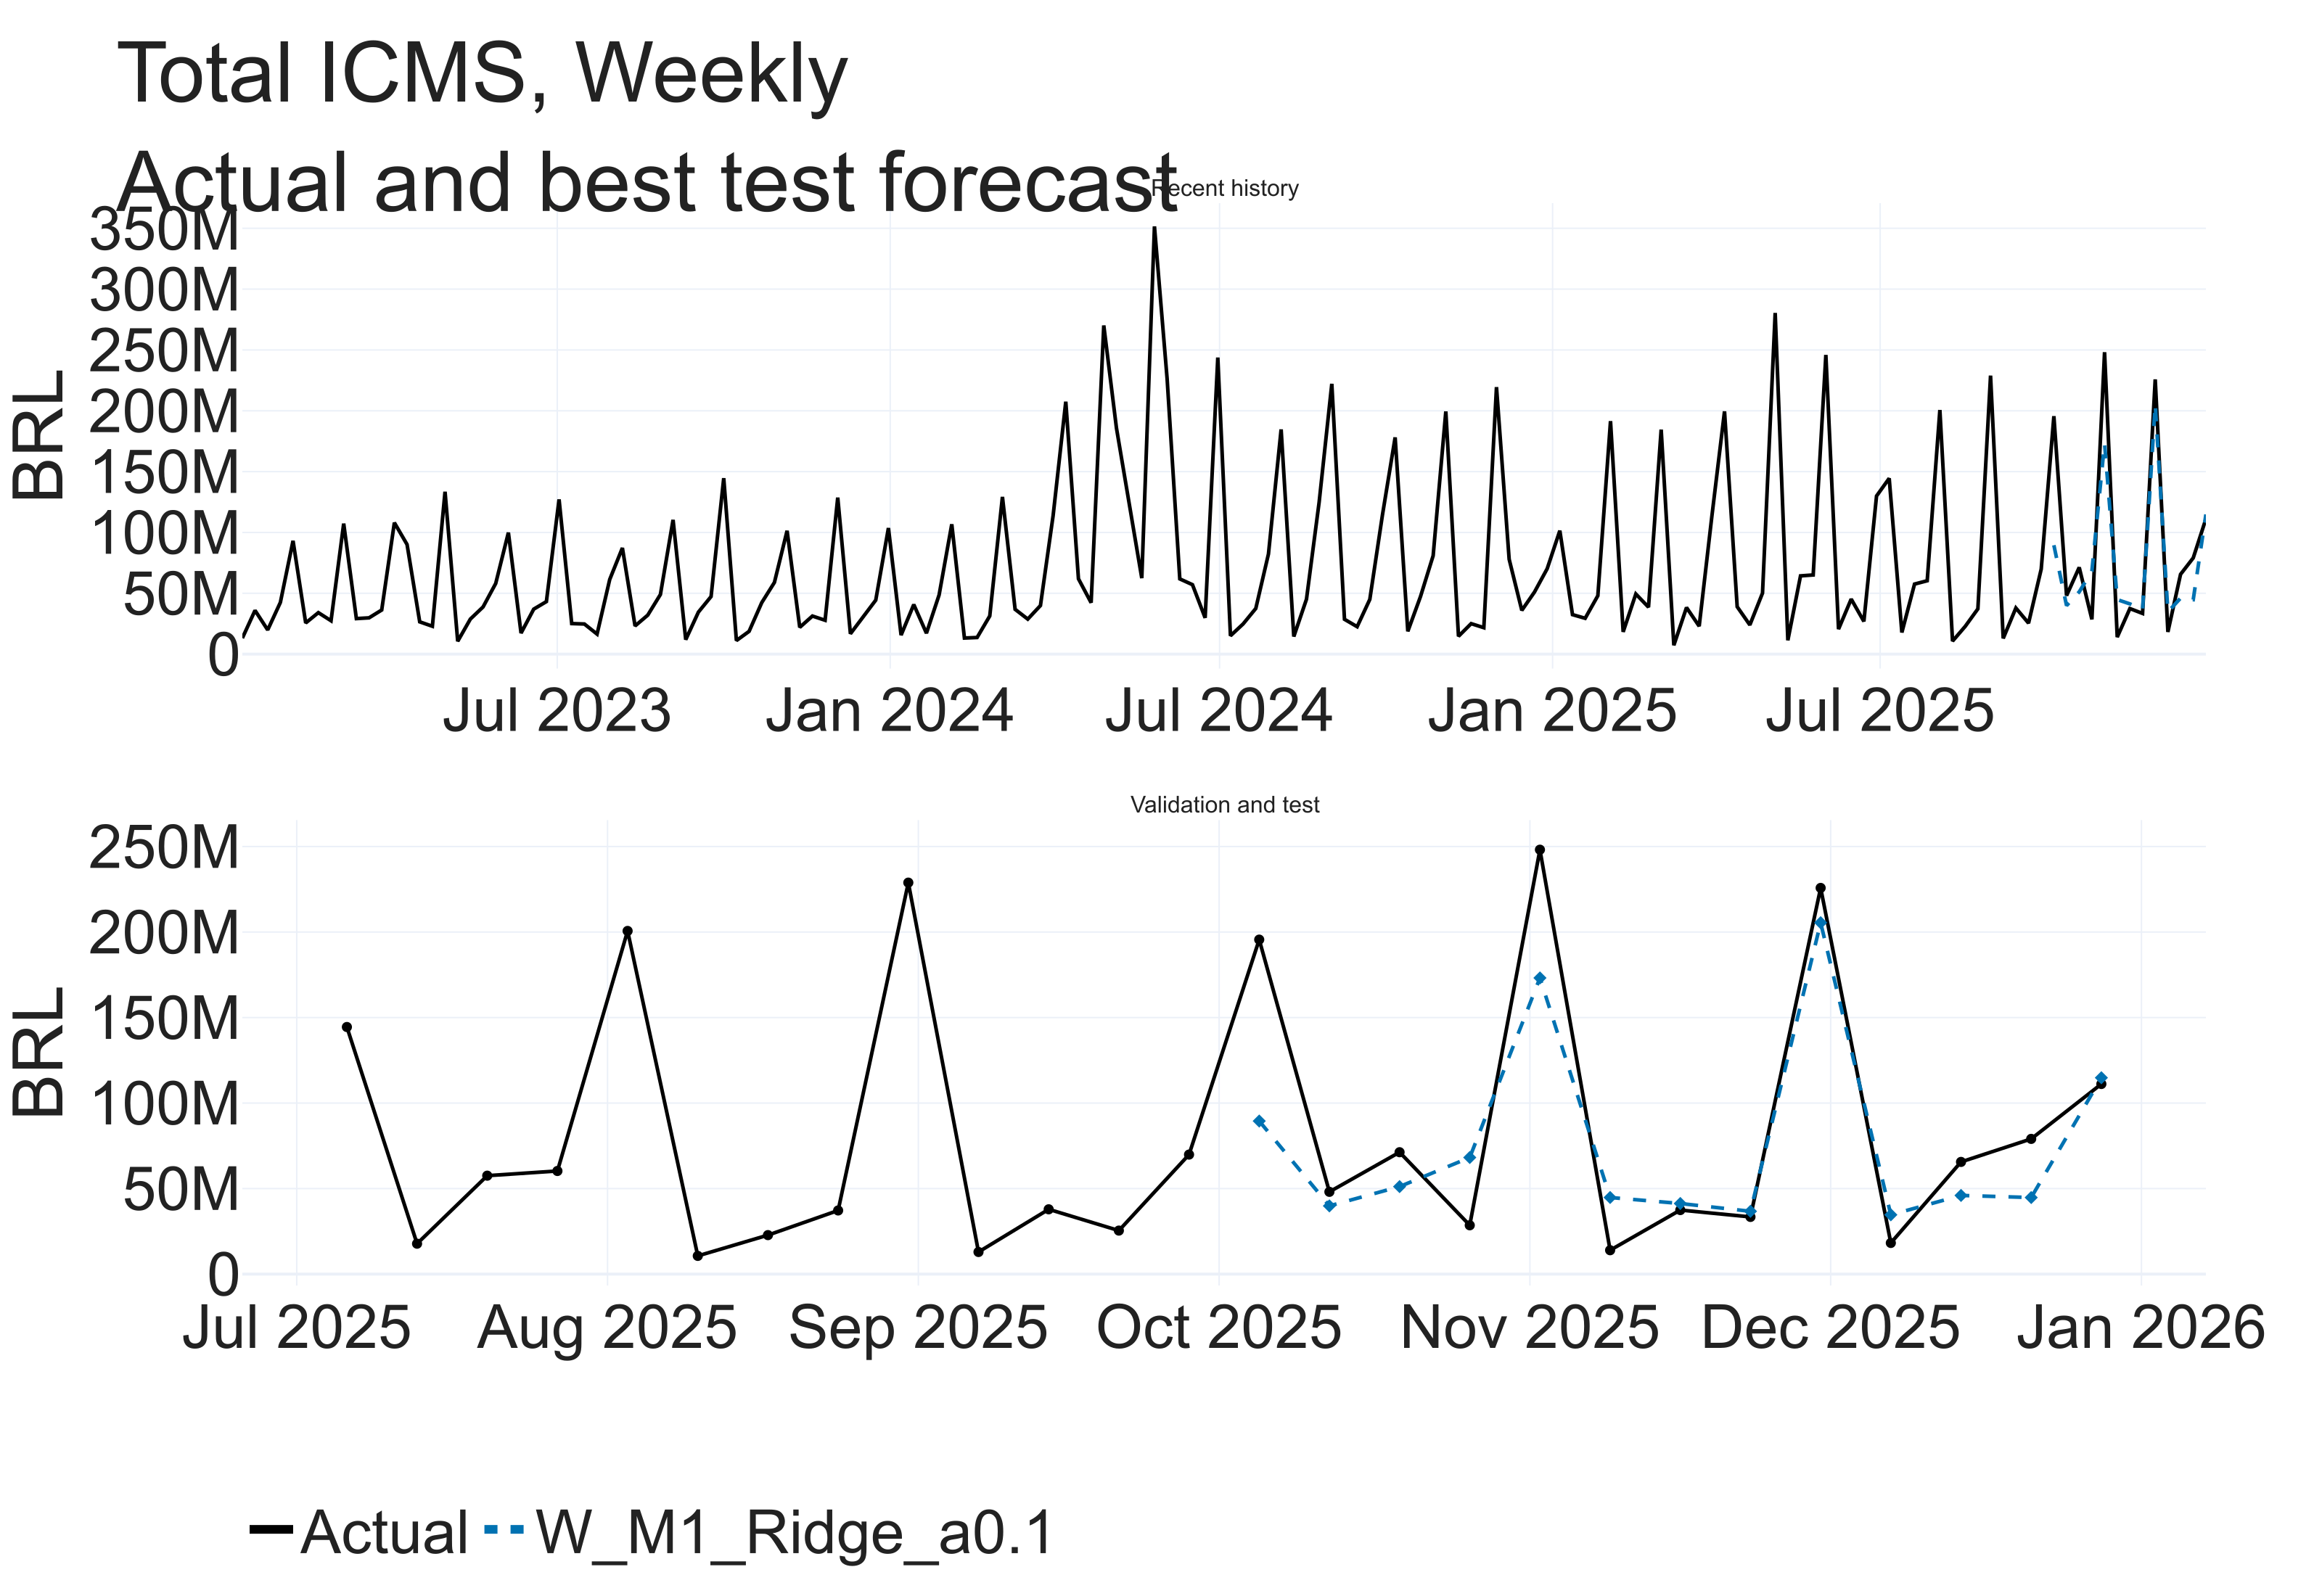
\includegraphics[width=\linewidth]{figures/segment/total_weekly_forecast.png}
  \caption{Total, weekly. Blue dashed: M1 ridge.}
\end{figure}
\begin{figure}[H]
  \centering
  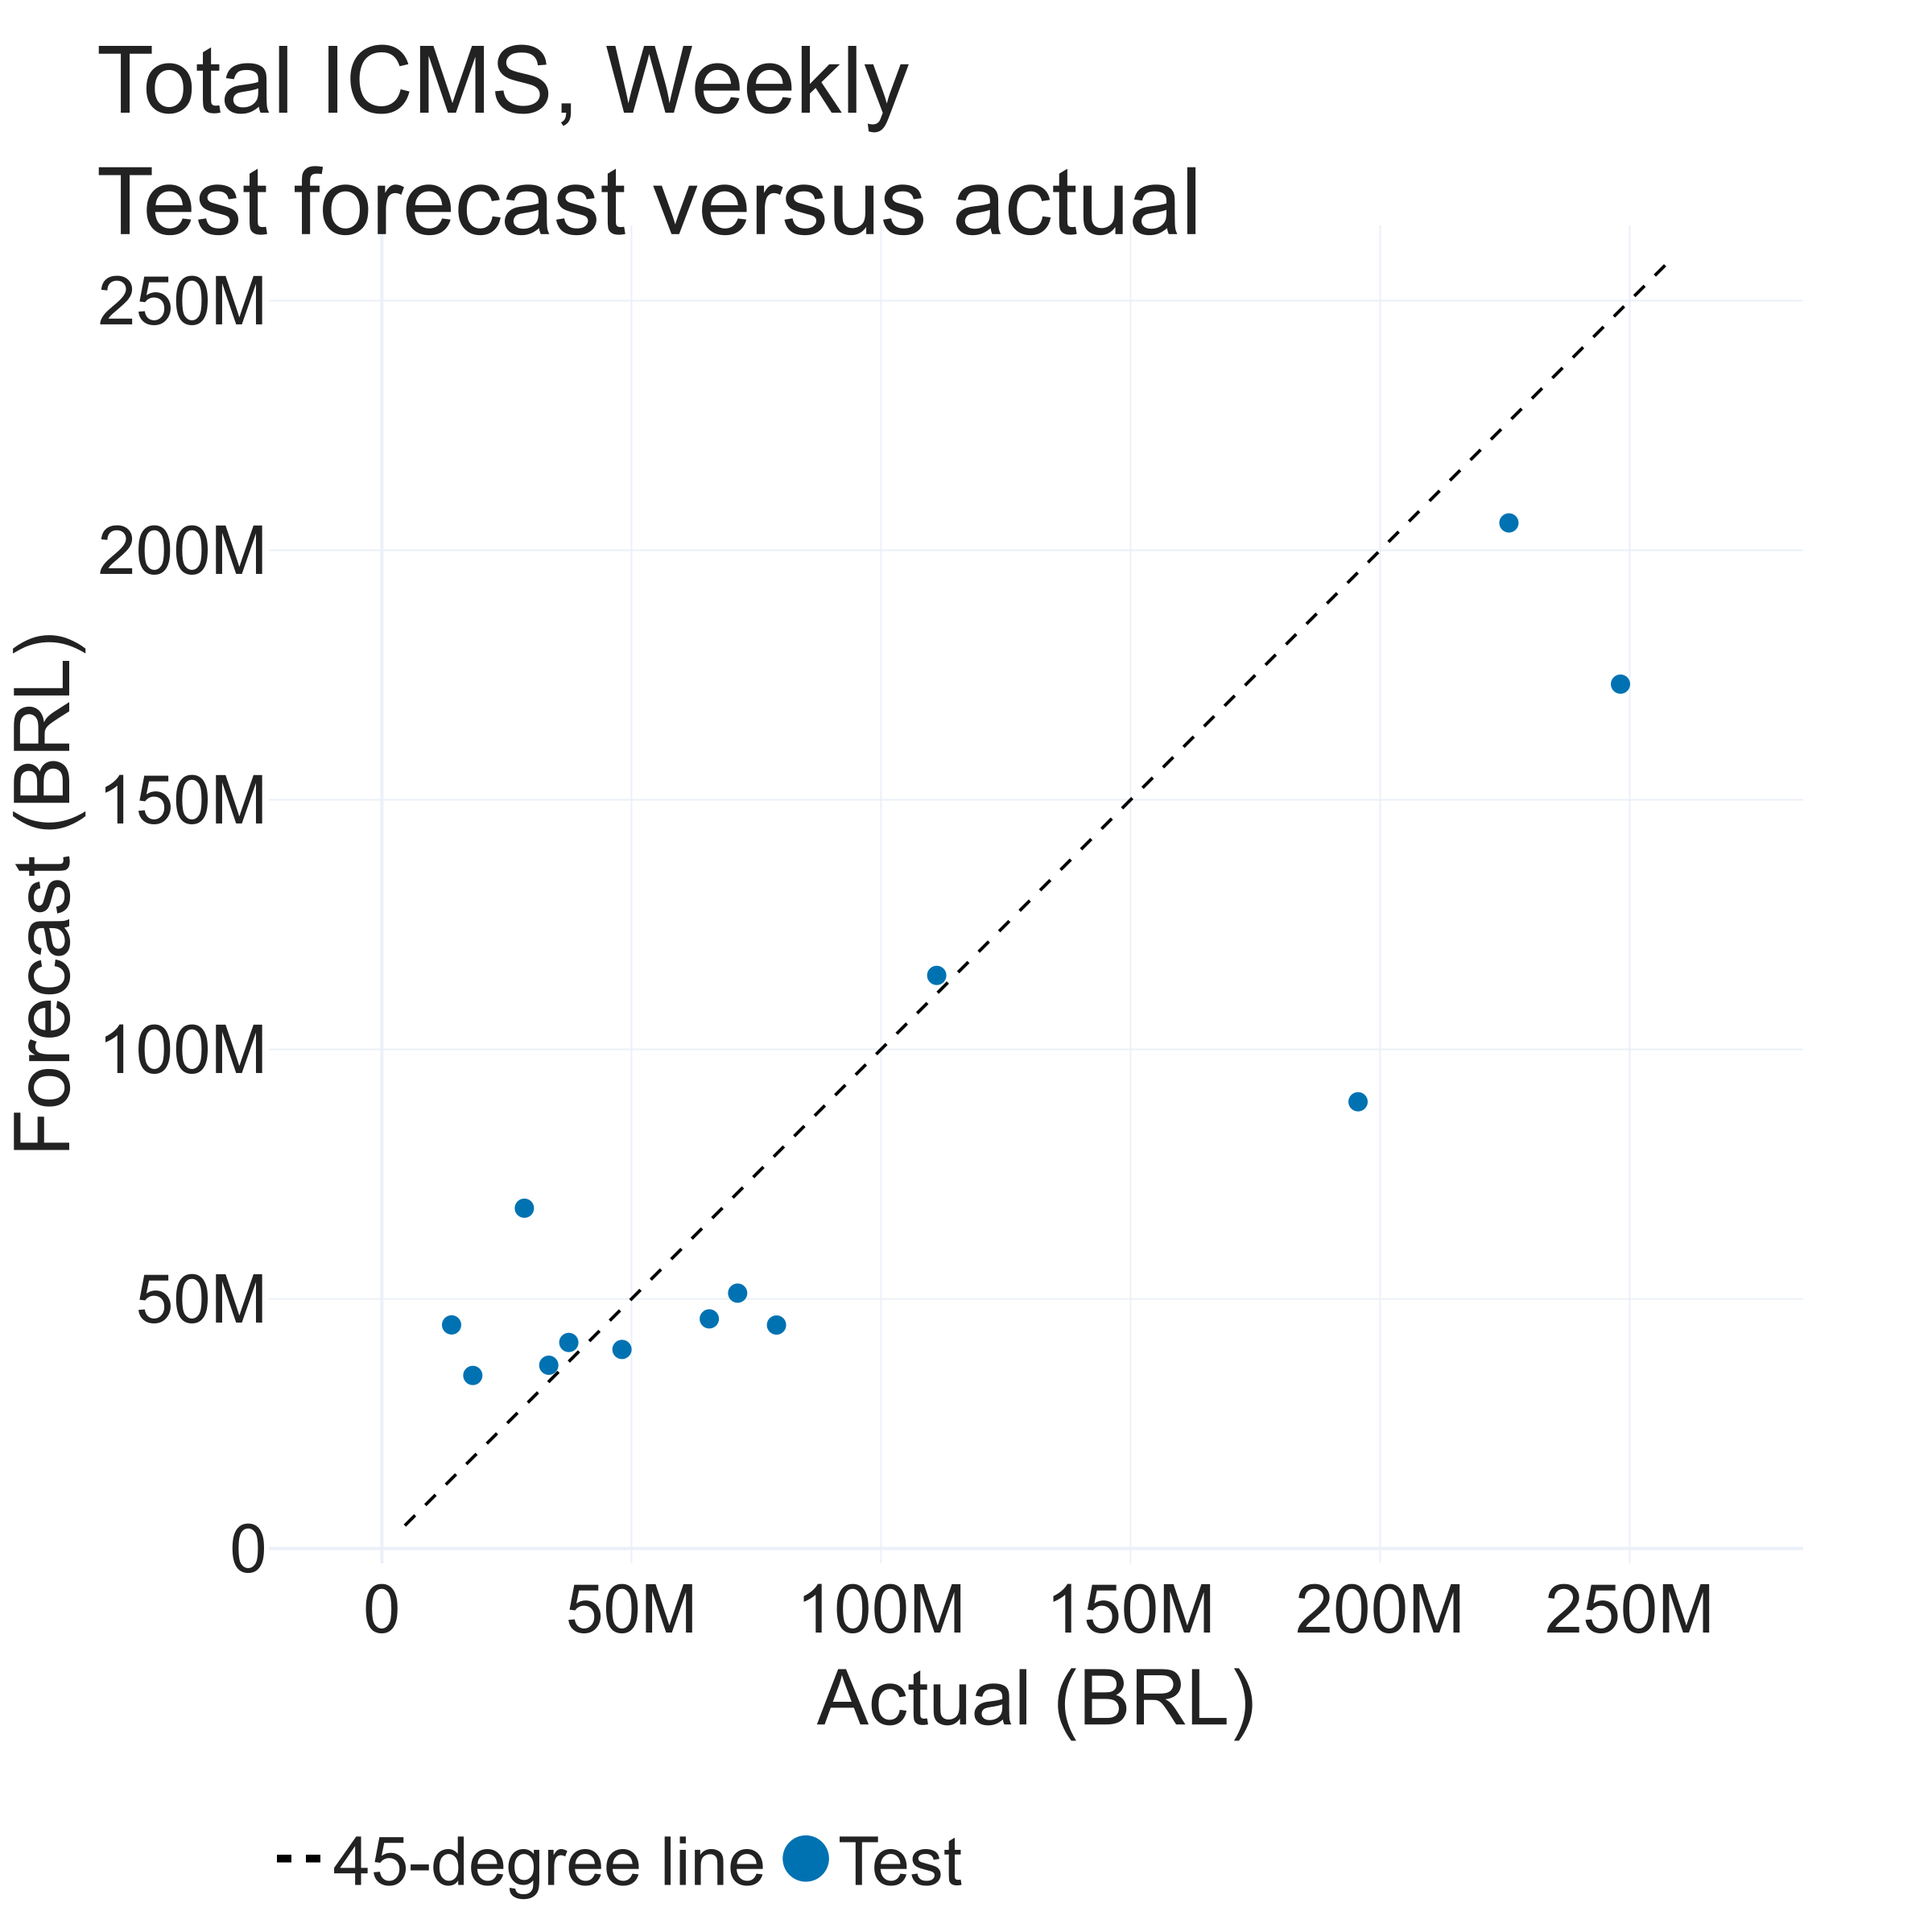
\includegraphics[width=0.62\linewidth]{figures/segment/total_weekly_scatter.png}
  \caption{Total, weekly test scatter.}
\end{figure}
\begin{figure}[H]
  \centering
  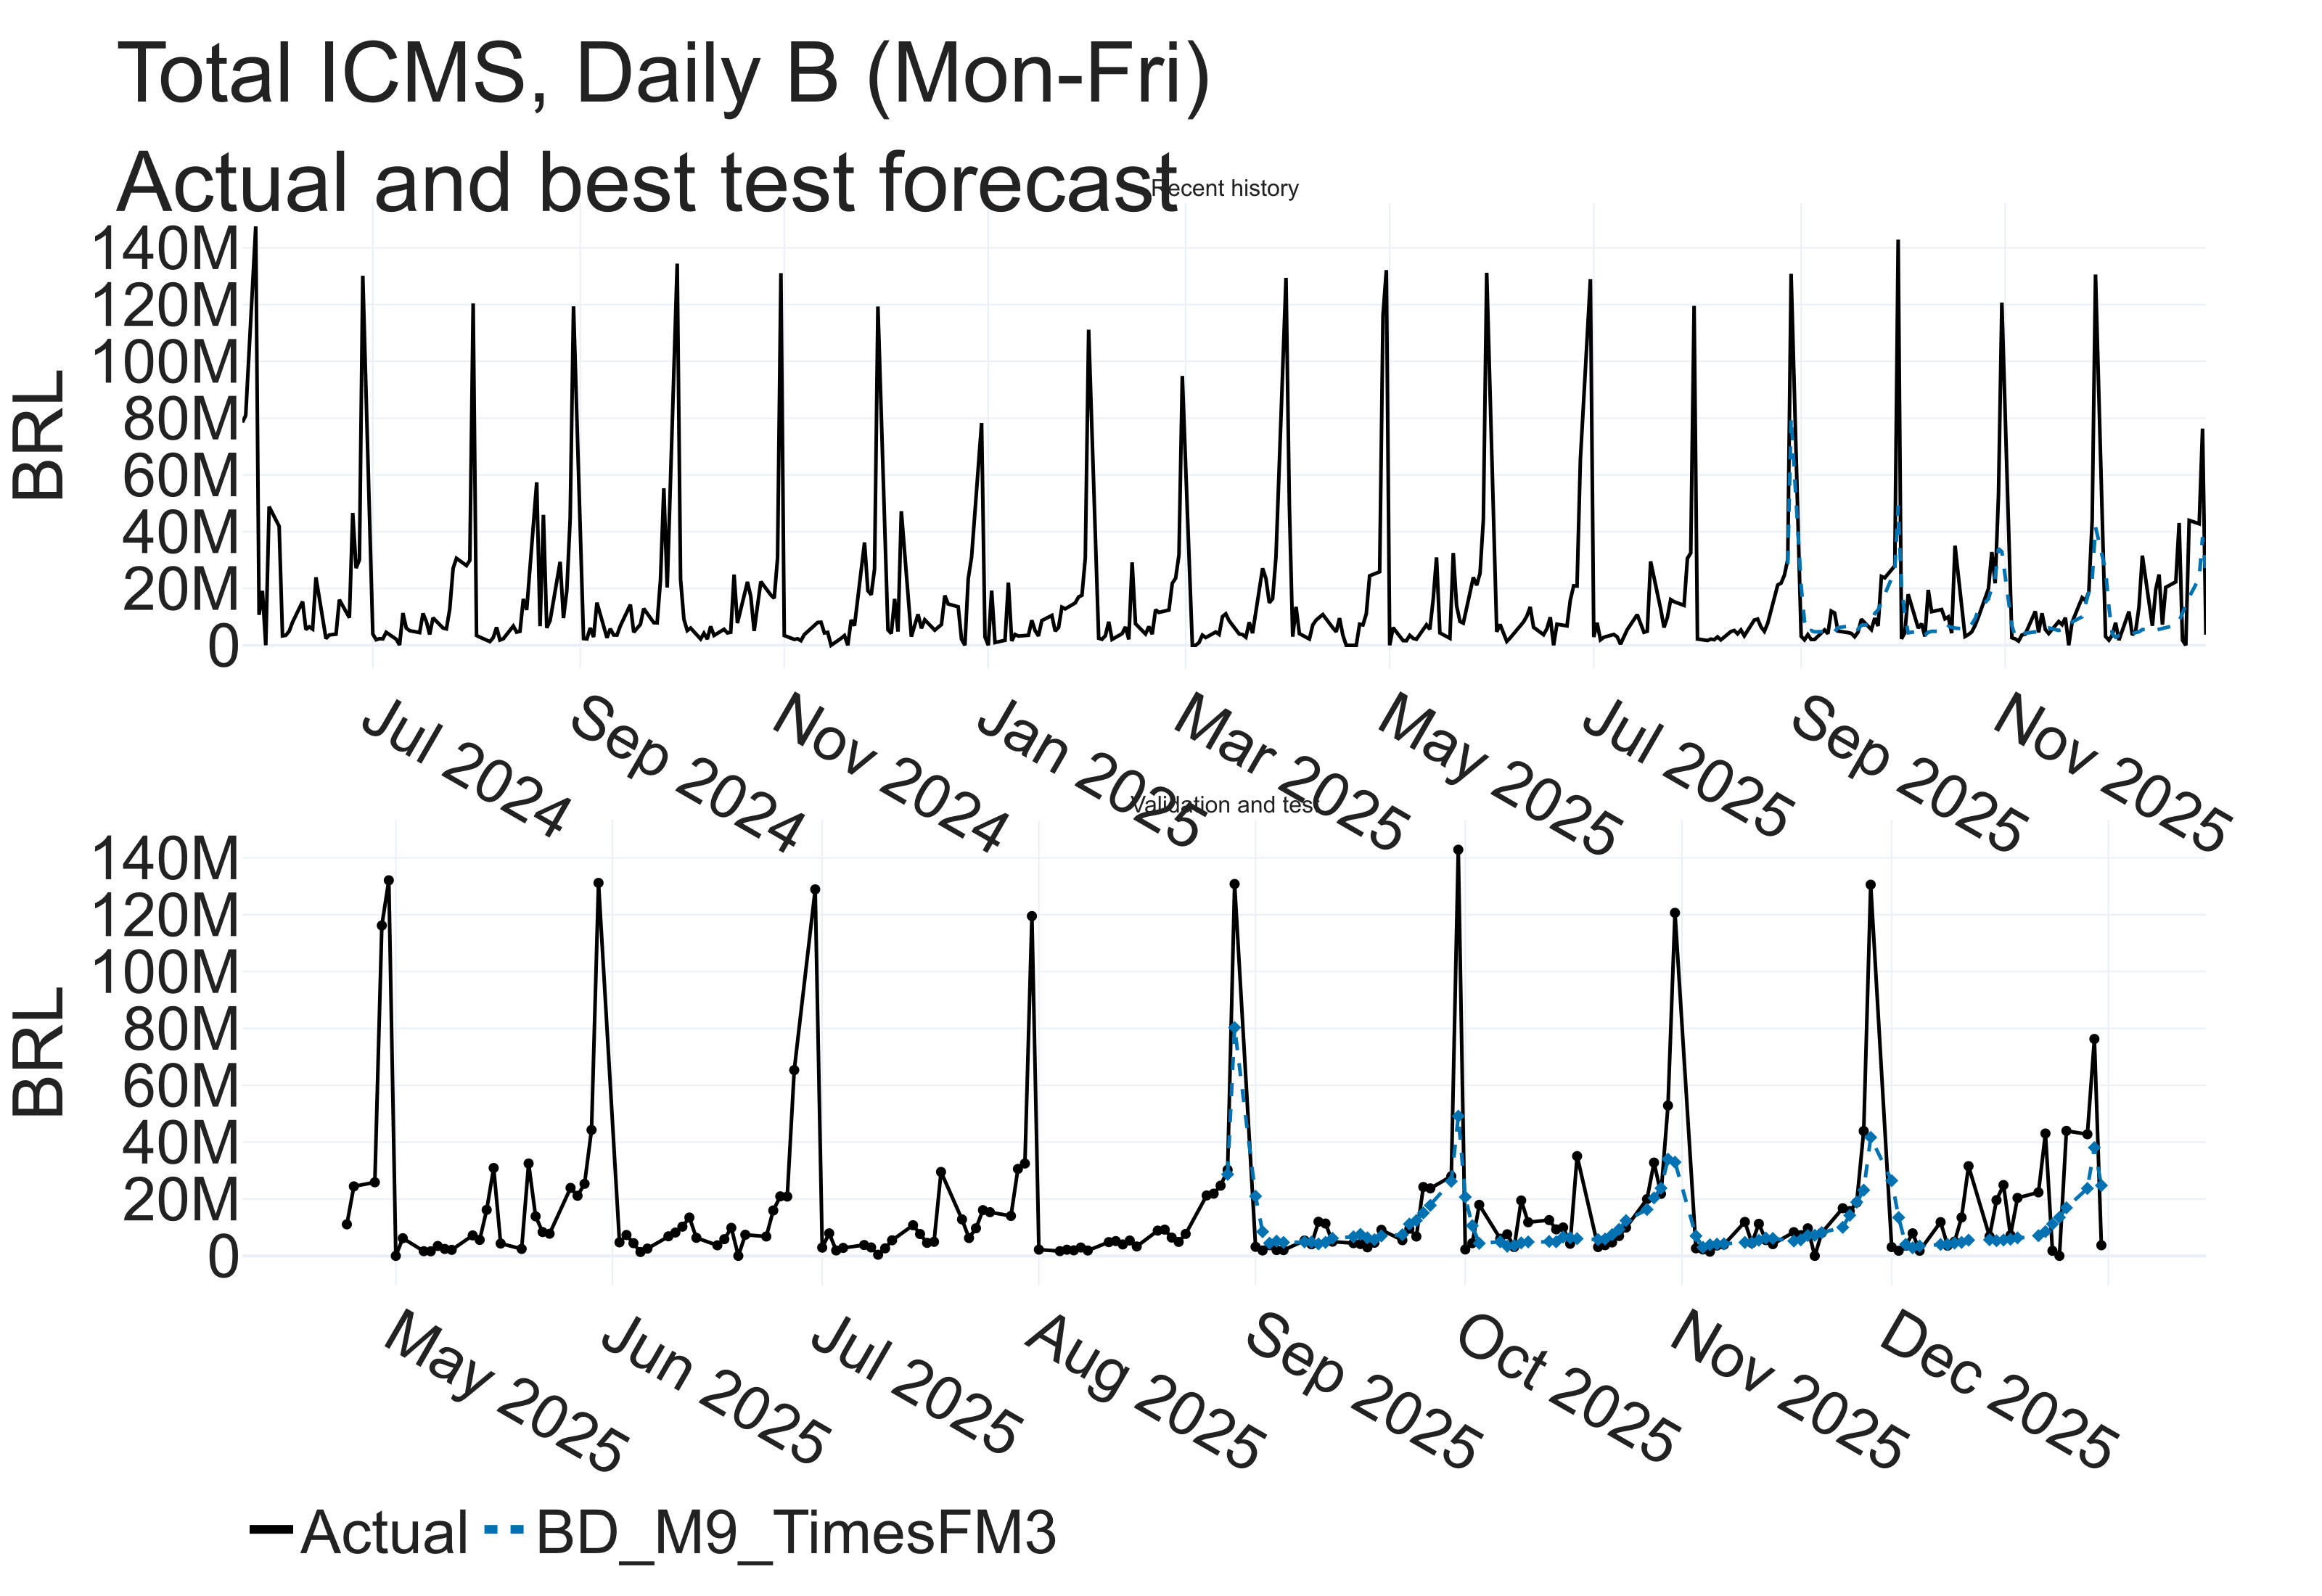
\includegraphics[width=\linewidth]{figures/segment/total_business_daily_forecast.png}
  \caption{Total, daily B. Blue dashed: M9 TimesFM.}
\end{figure}
\begin{figure}[H]
  \centering
  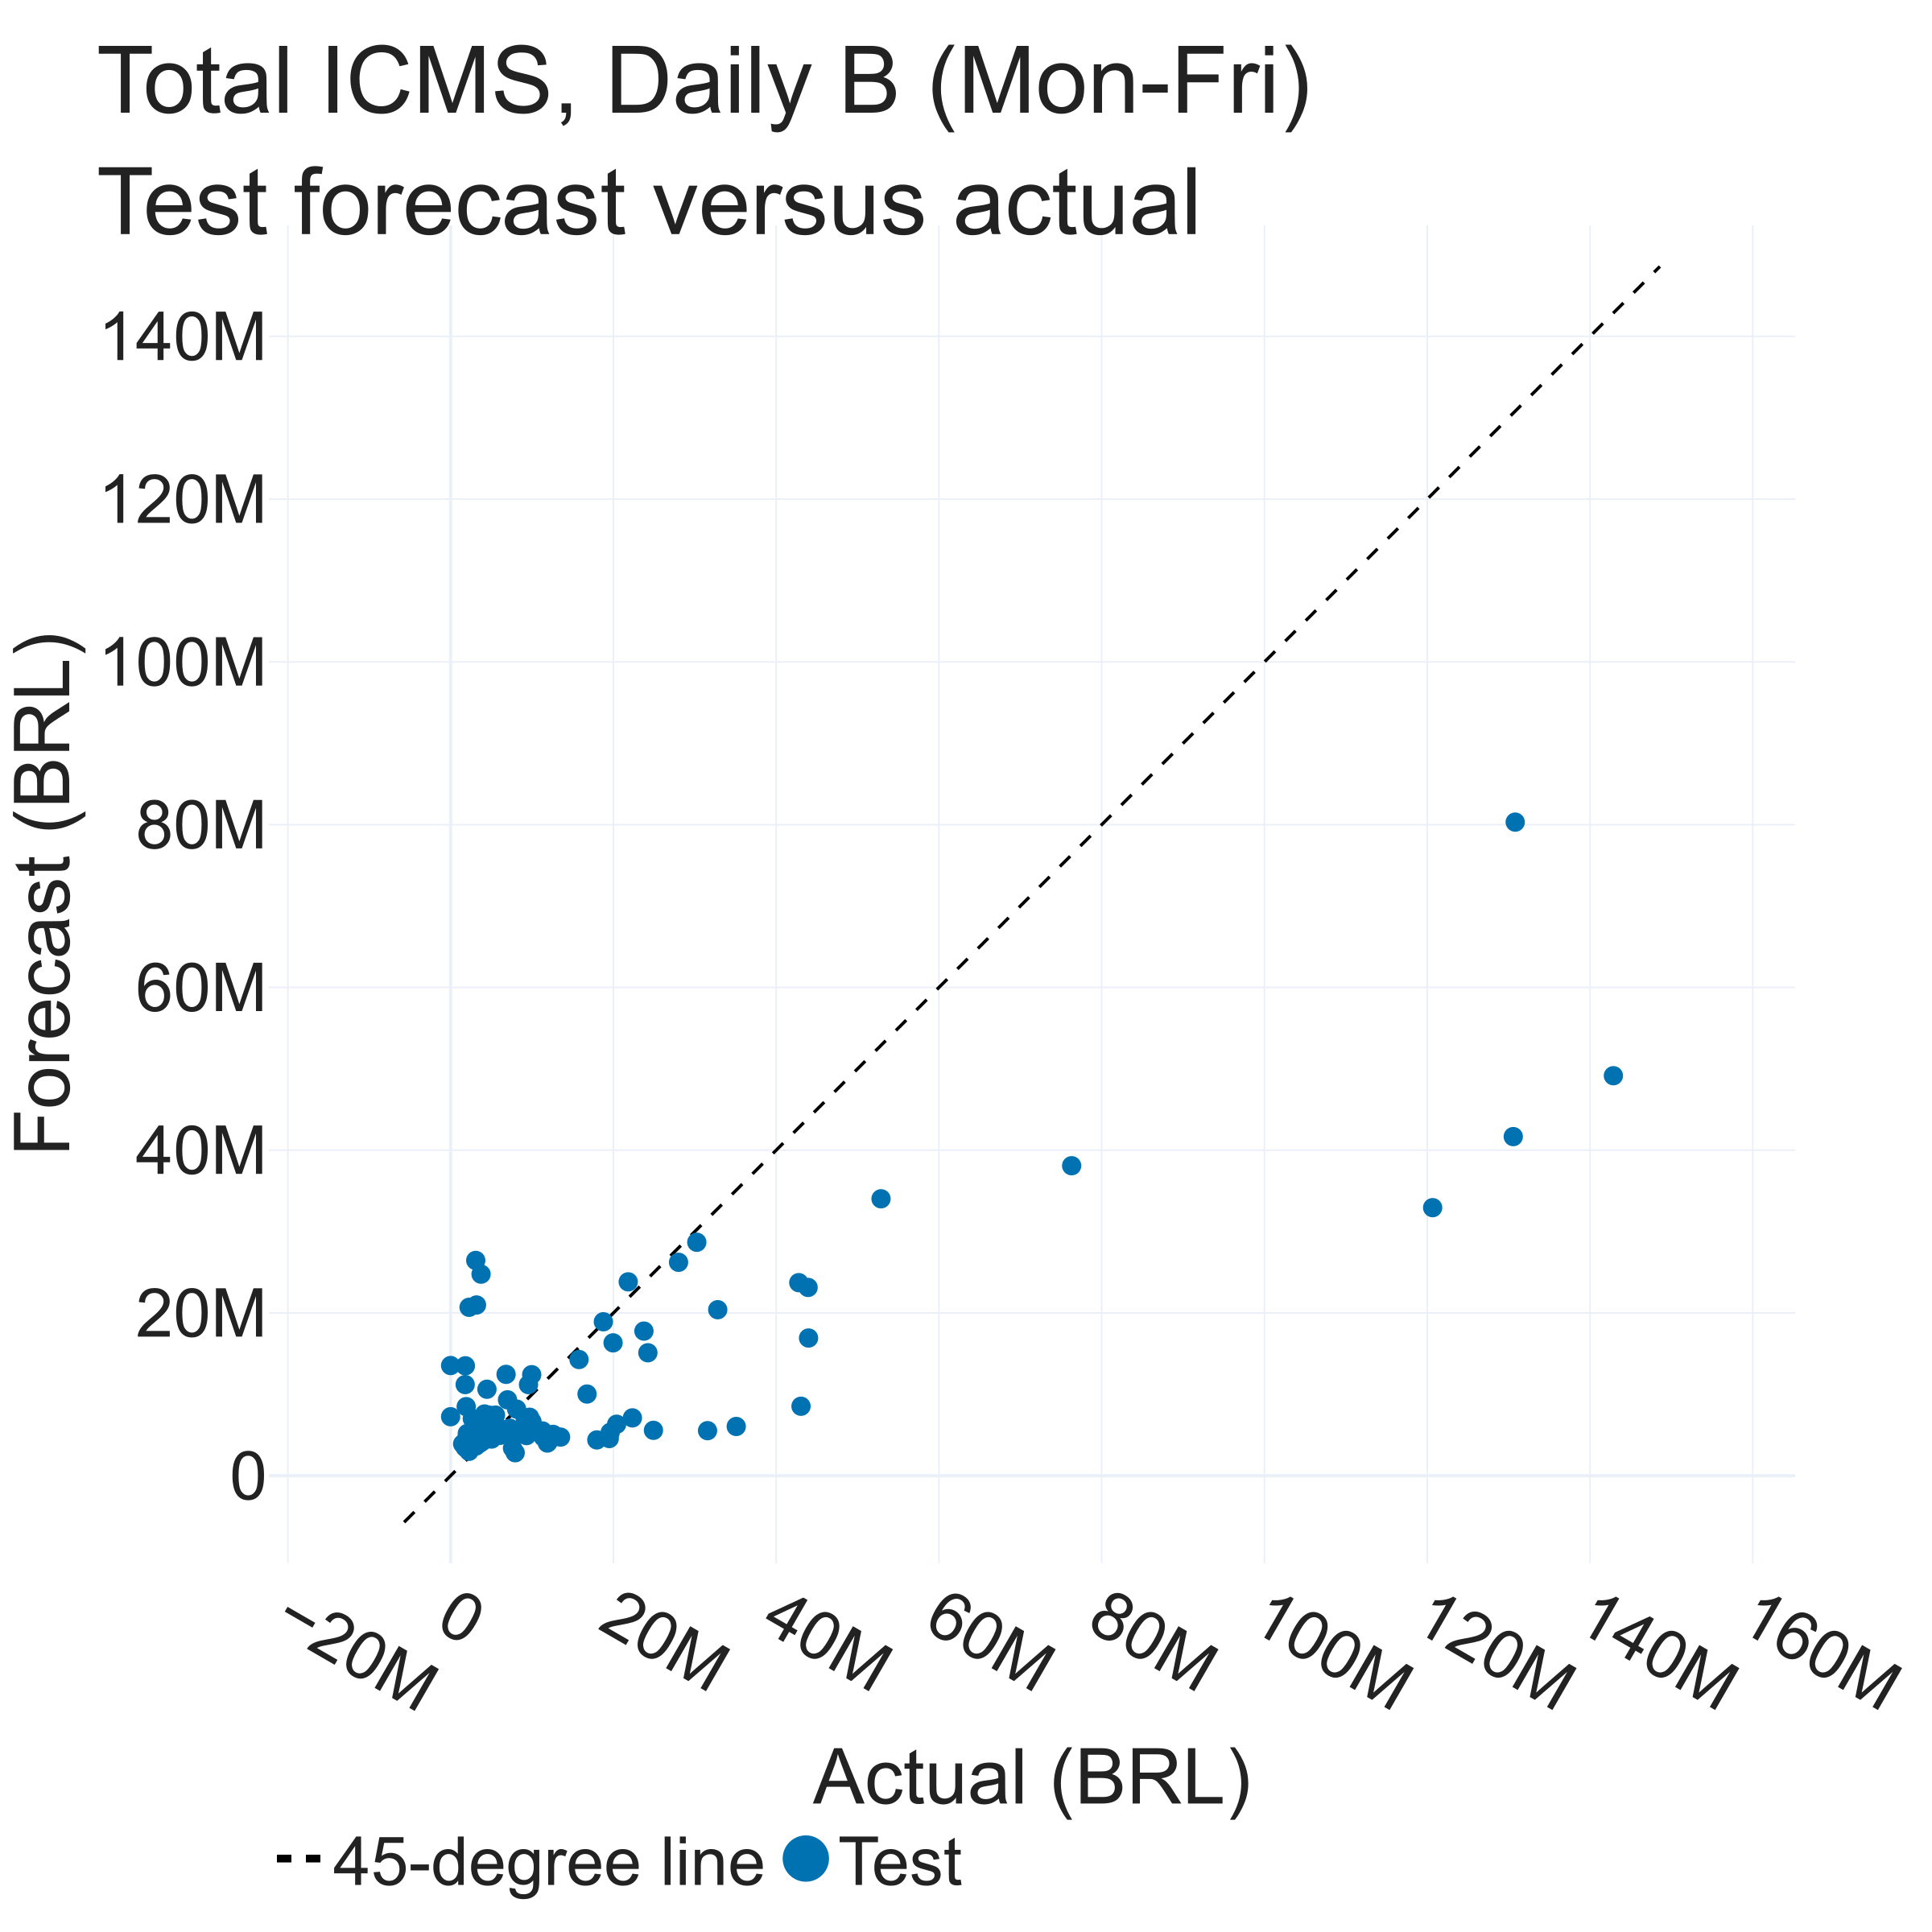
\includegraphics[width=0.62\linewidth]{figures/segment/total_business_daily_scatter.png}
  \caption{Total, daily B test scatter.}
\end{figure}
\begin{figure}[H]
  \centering
  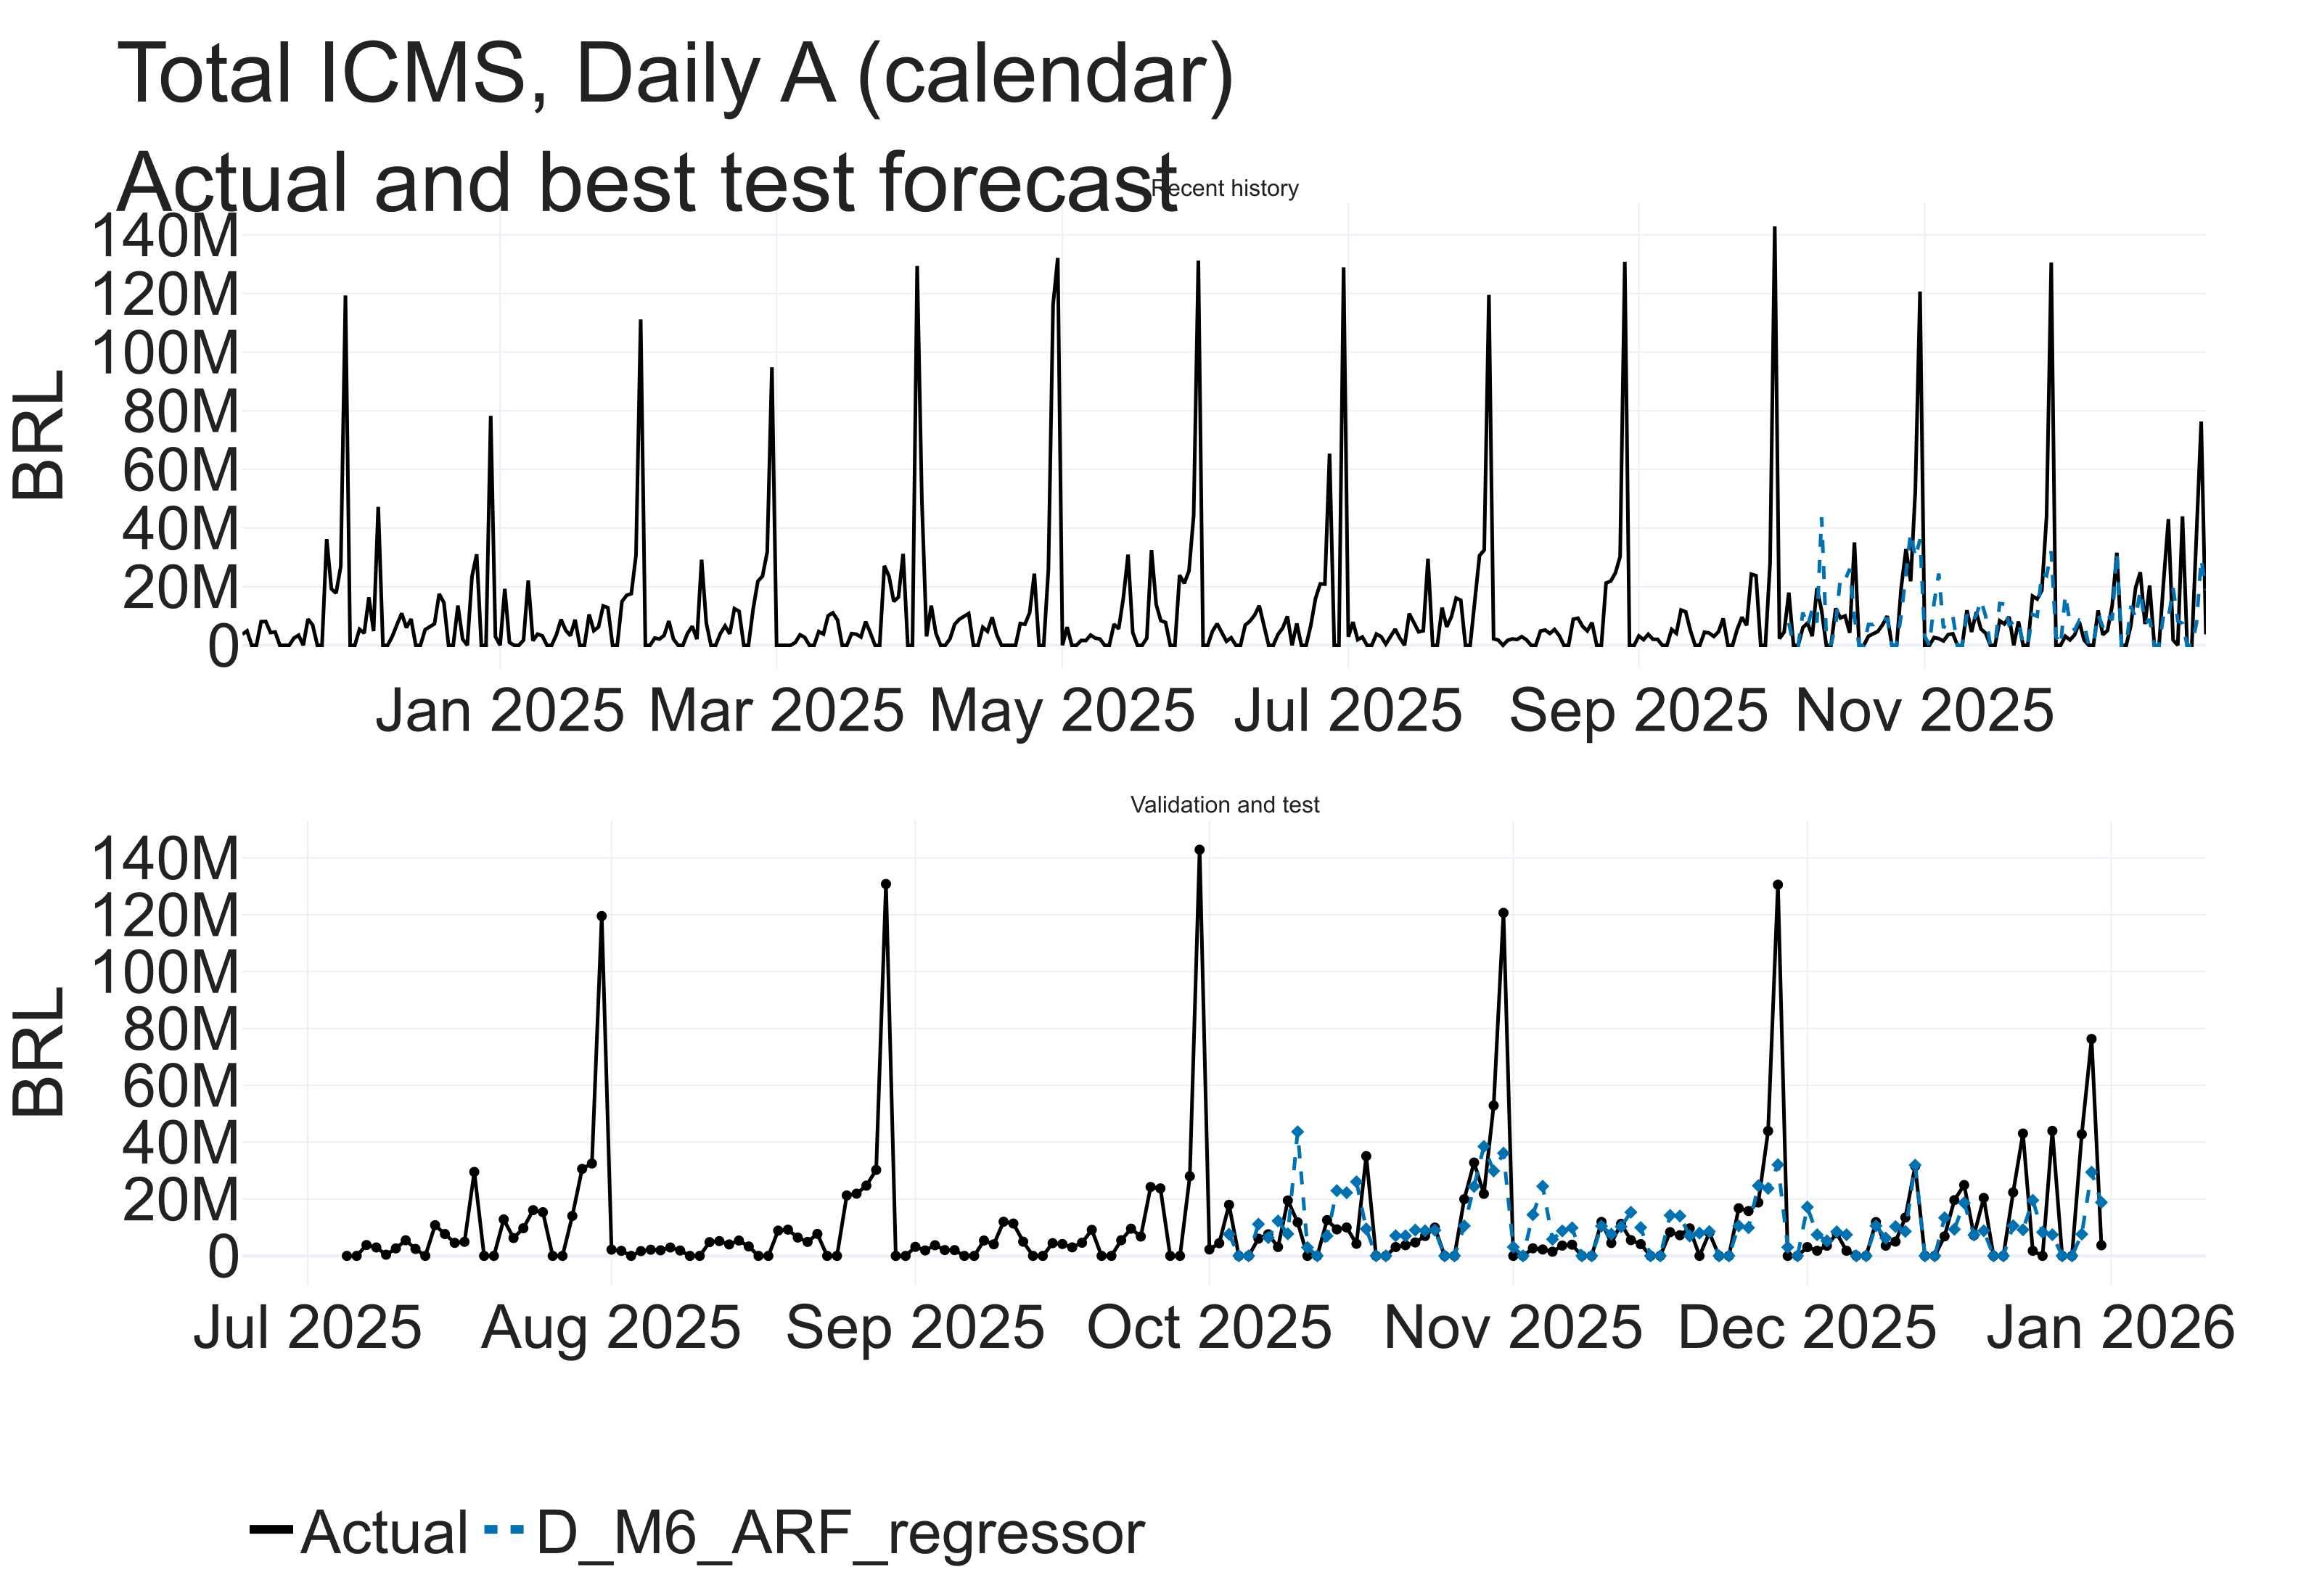
\includegraphics[width=\linewidth]{figures/segment/total_daily_forecast.png}
  \caption{Total, daily A. Blue dashed: M6 forest.}
\end{figure}
\begin{figure}[H]
  \centering
  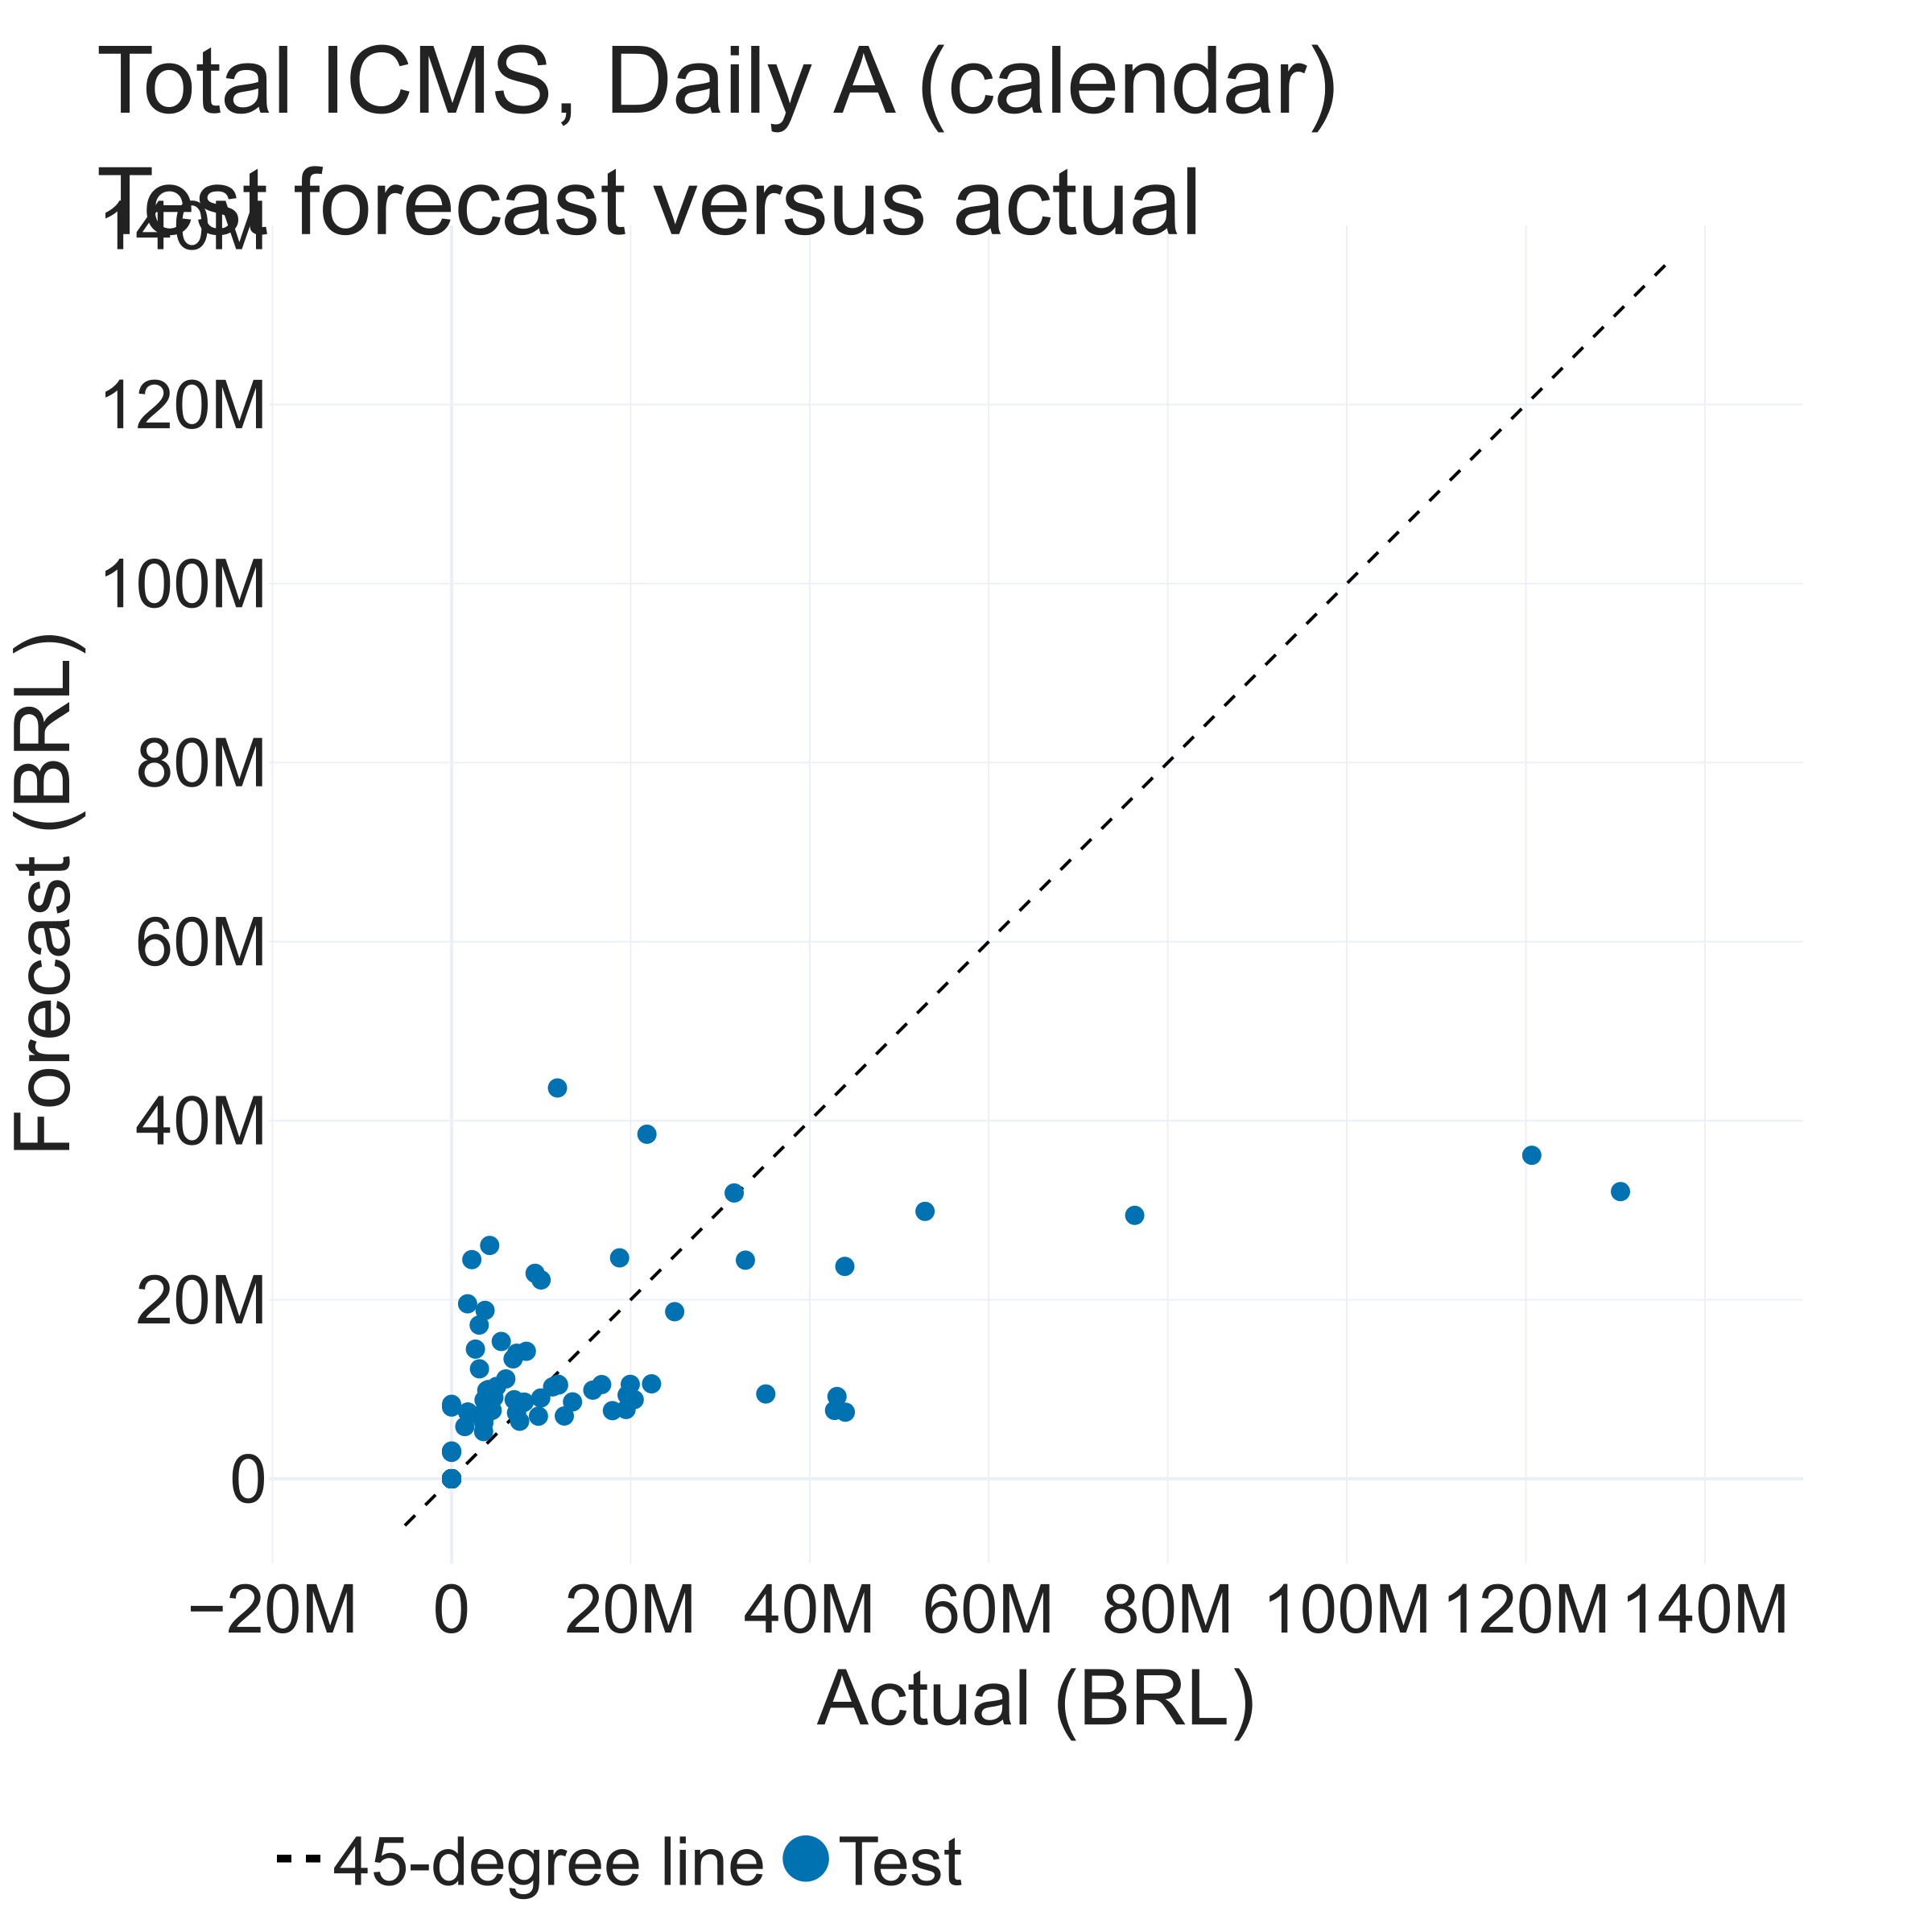
\includegraphics[width=0.62\linewidth]{figures/segment/total_daily_scatter.png}
  \caption{Total, daily A test scatter.}
\end{figure}
\begin{figure}[H]
  \centering
  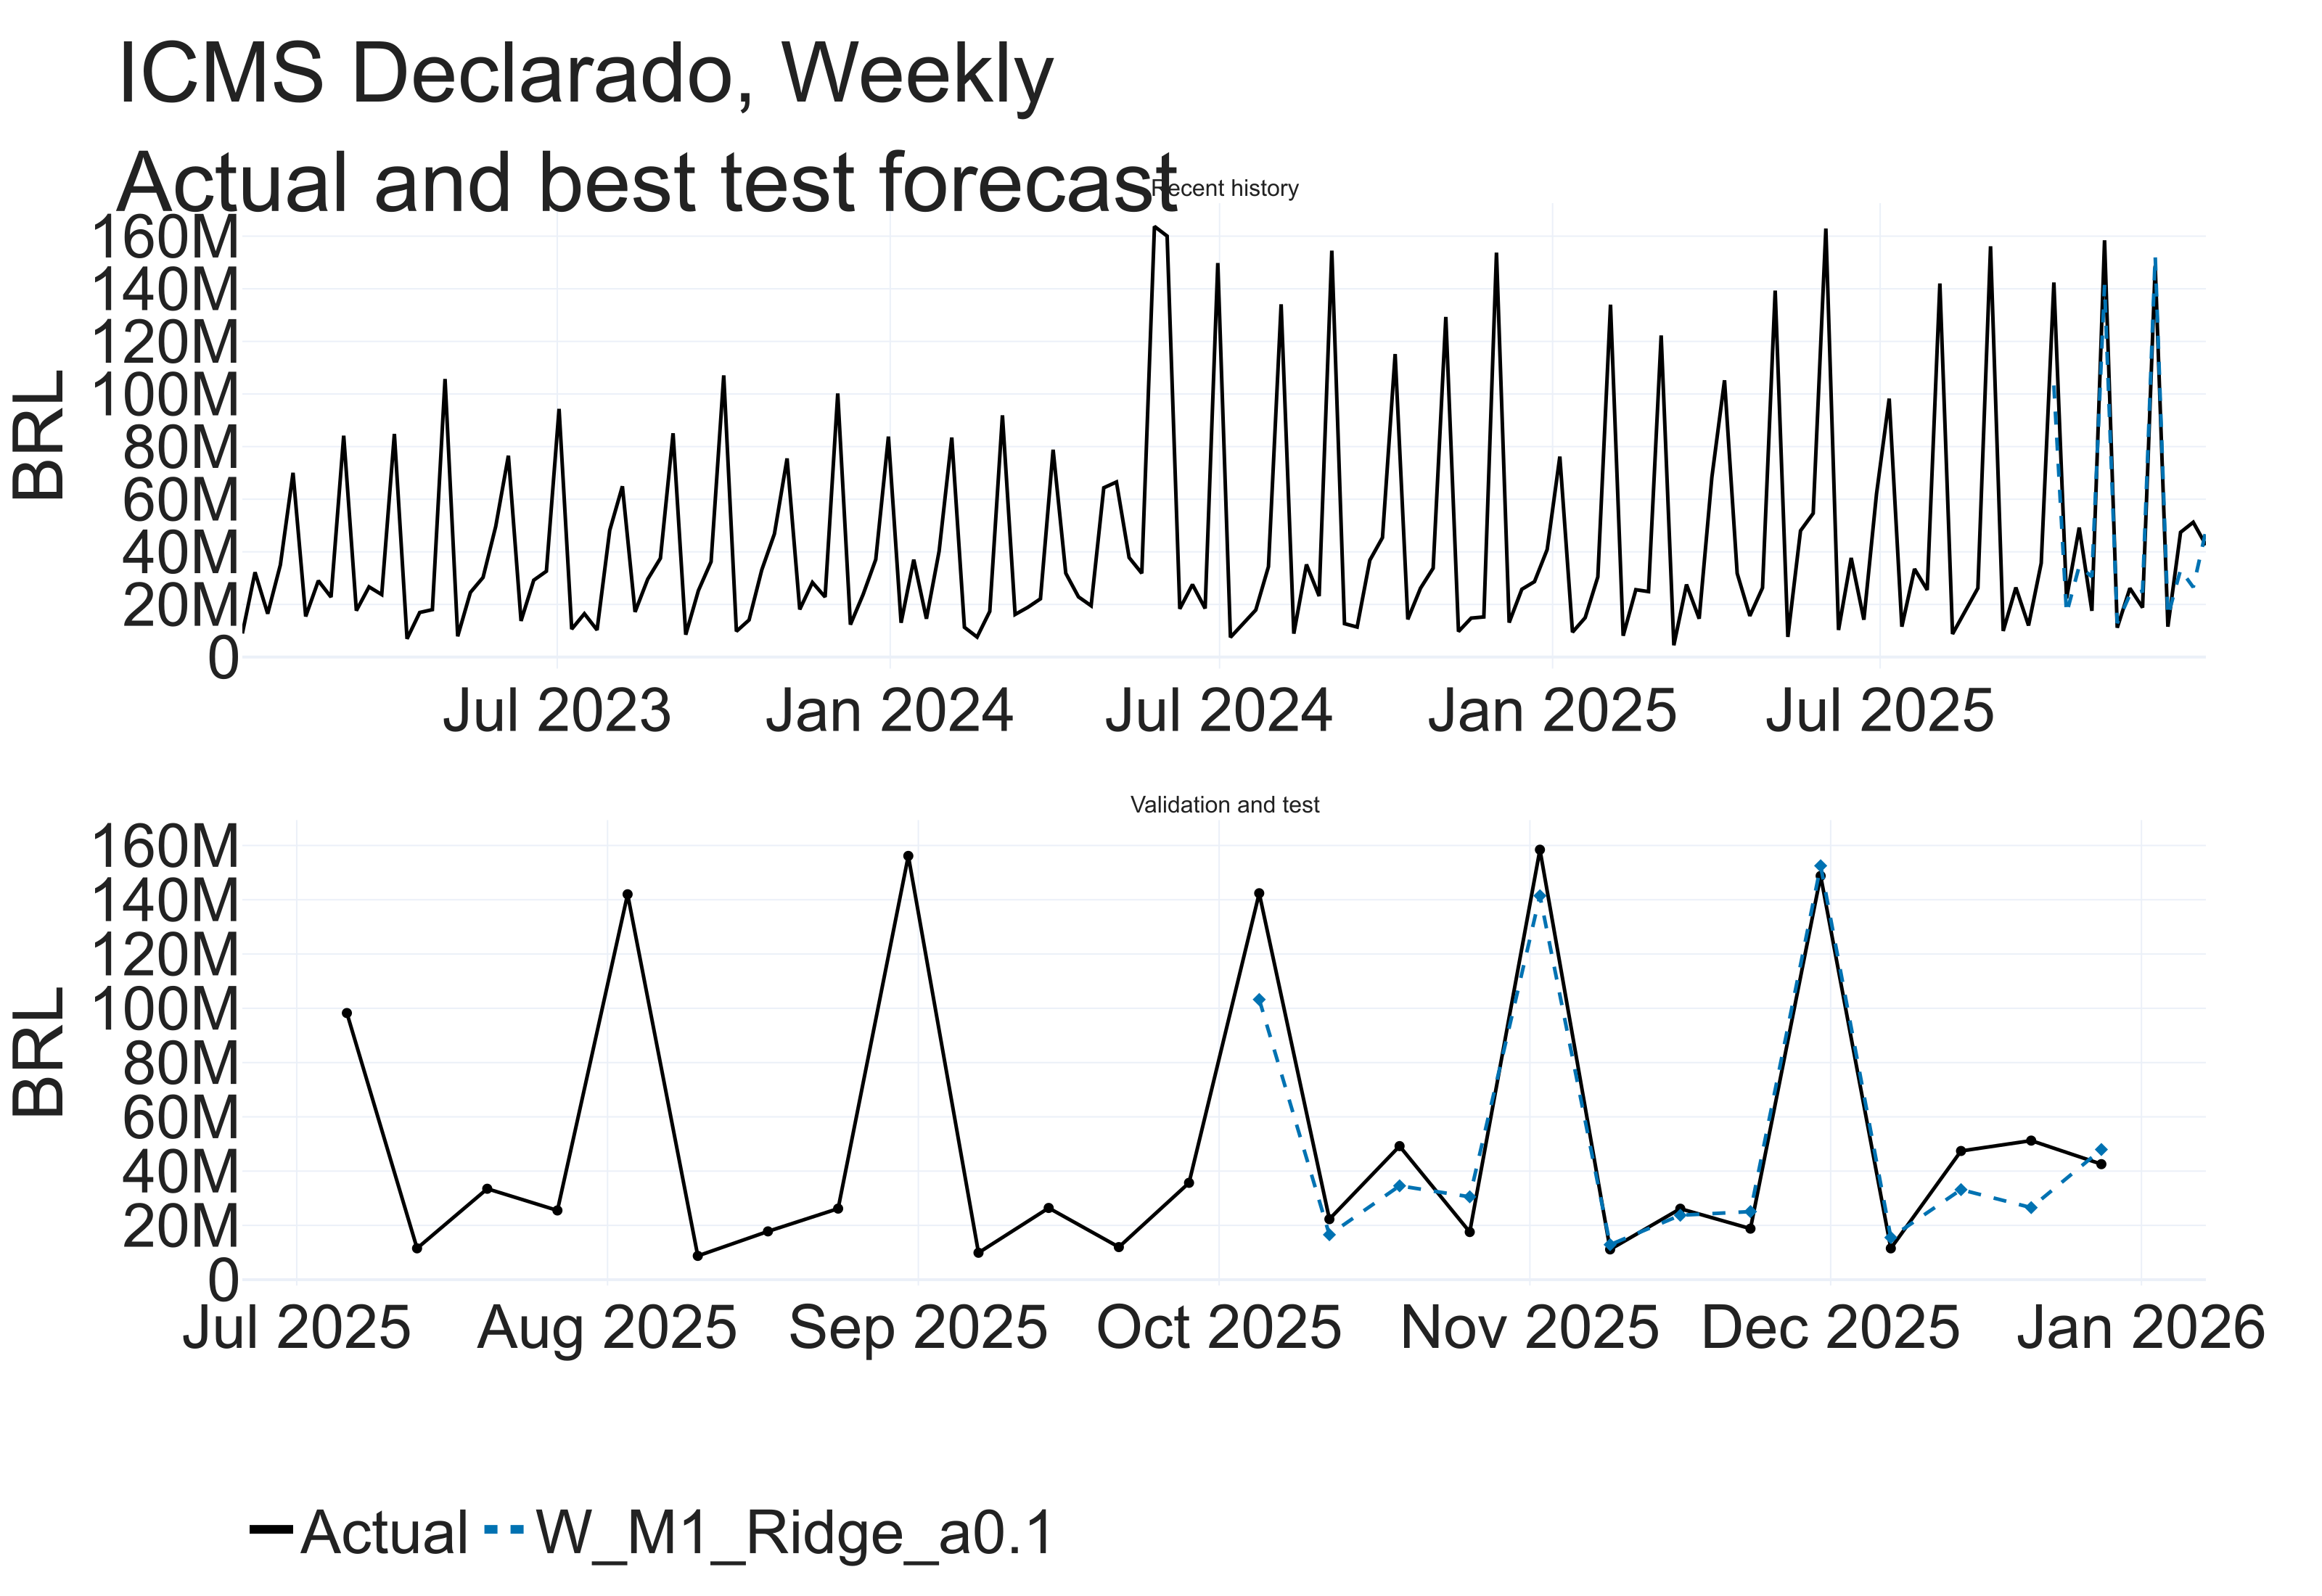
\includegraphics[width=\linewidth]{figures/segment/declarado_weekly_forecast.png}
  \caption{Declarado, weekly. Blue dashed: M1 ridge.}
\end{figure}
\begin{figure}[H]
  \centering
  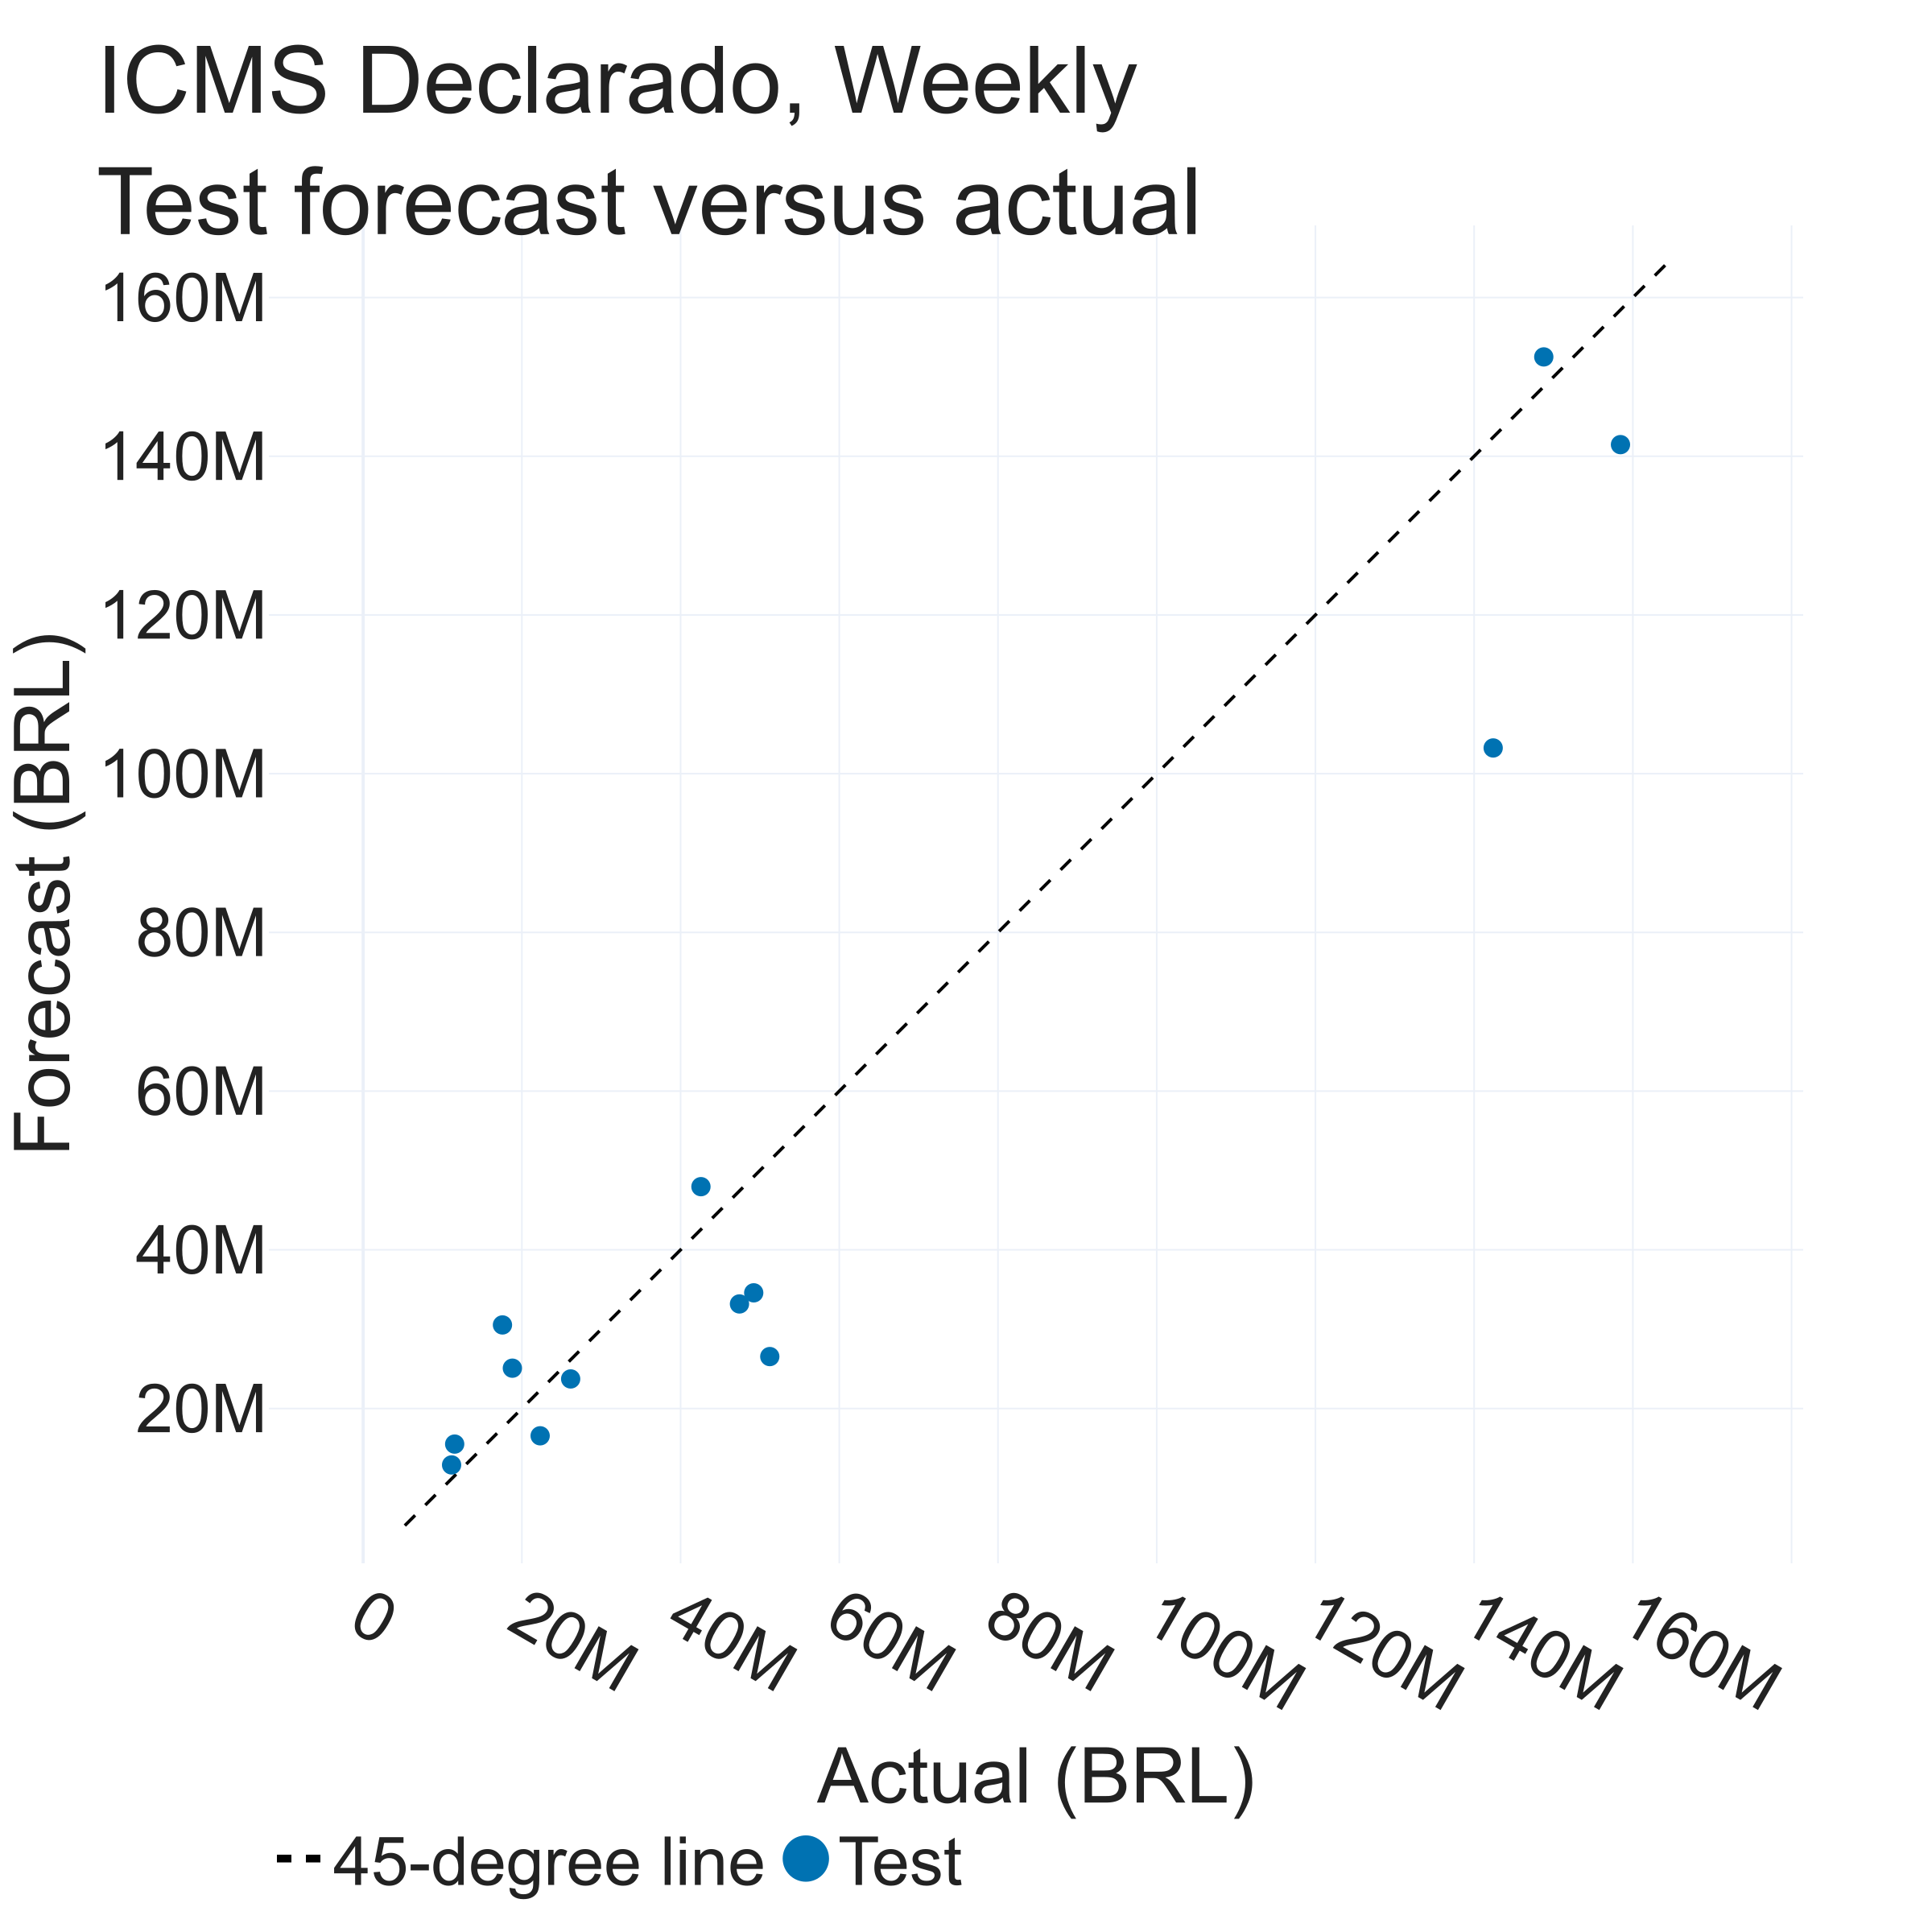
\includegraphics[width=0.62\linewidth]{figures/segment/declarado_weekly_scatter.png}
  \caption{Declarado, weekly test scatter.}
\end{figure}
\begin{figure}[H]
  \centering
  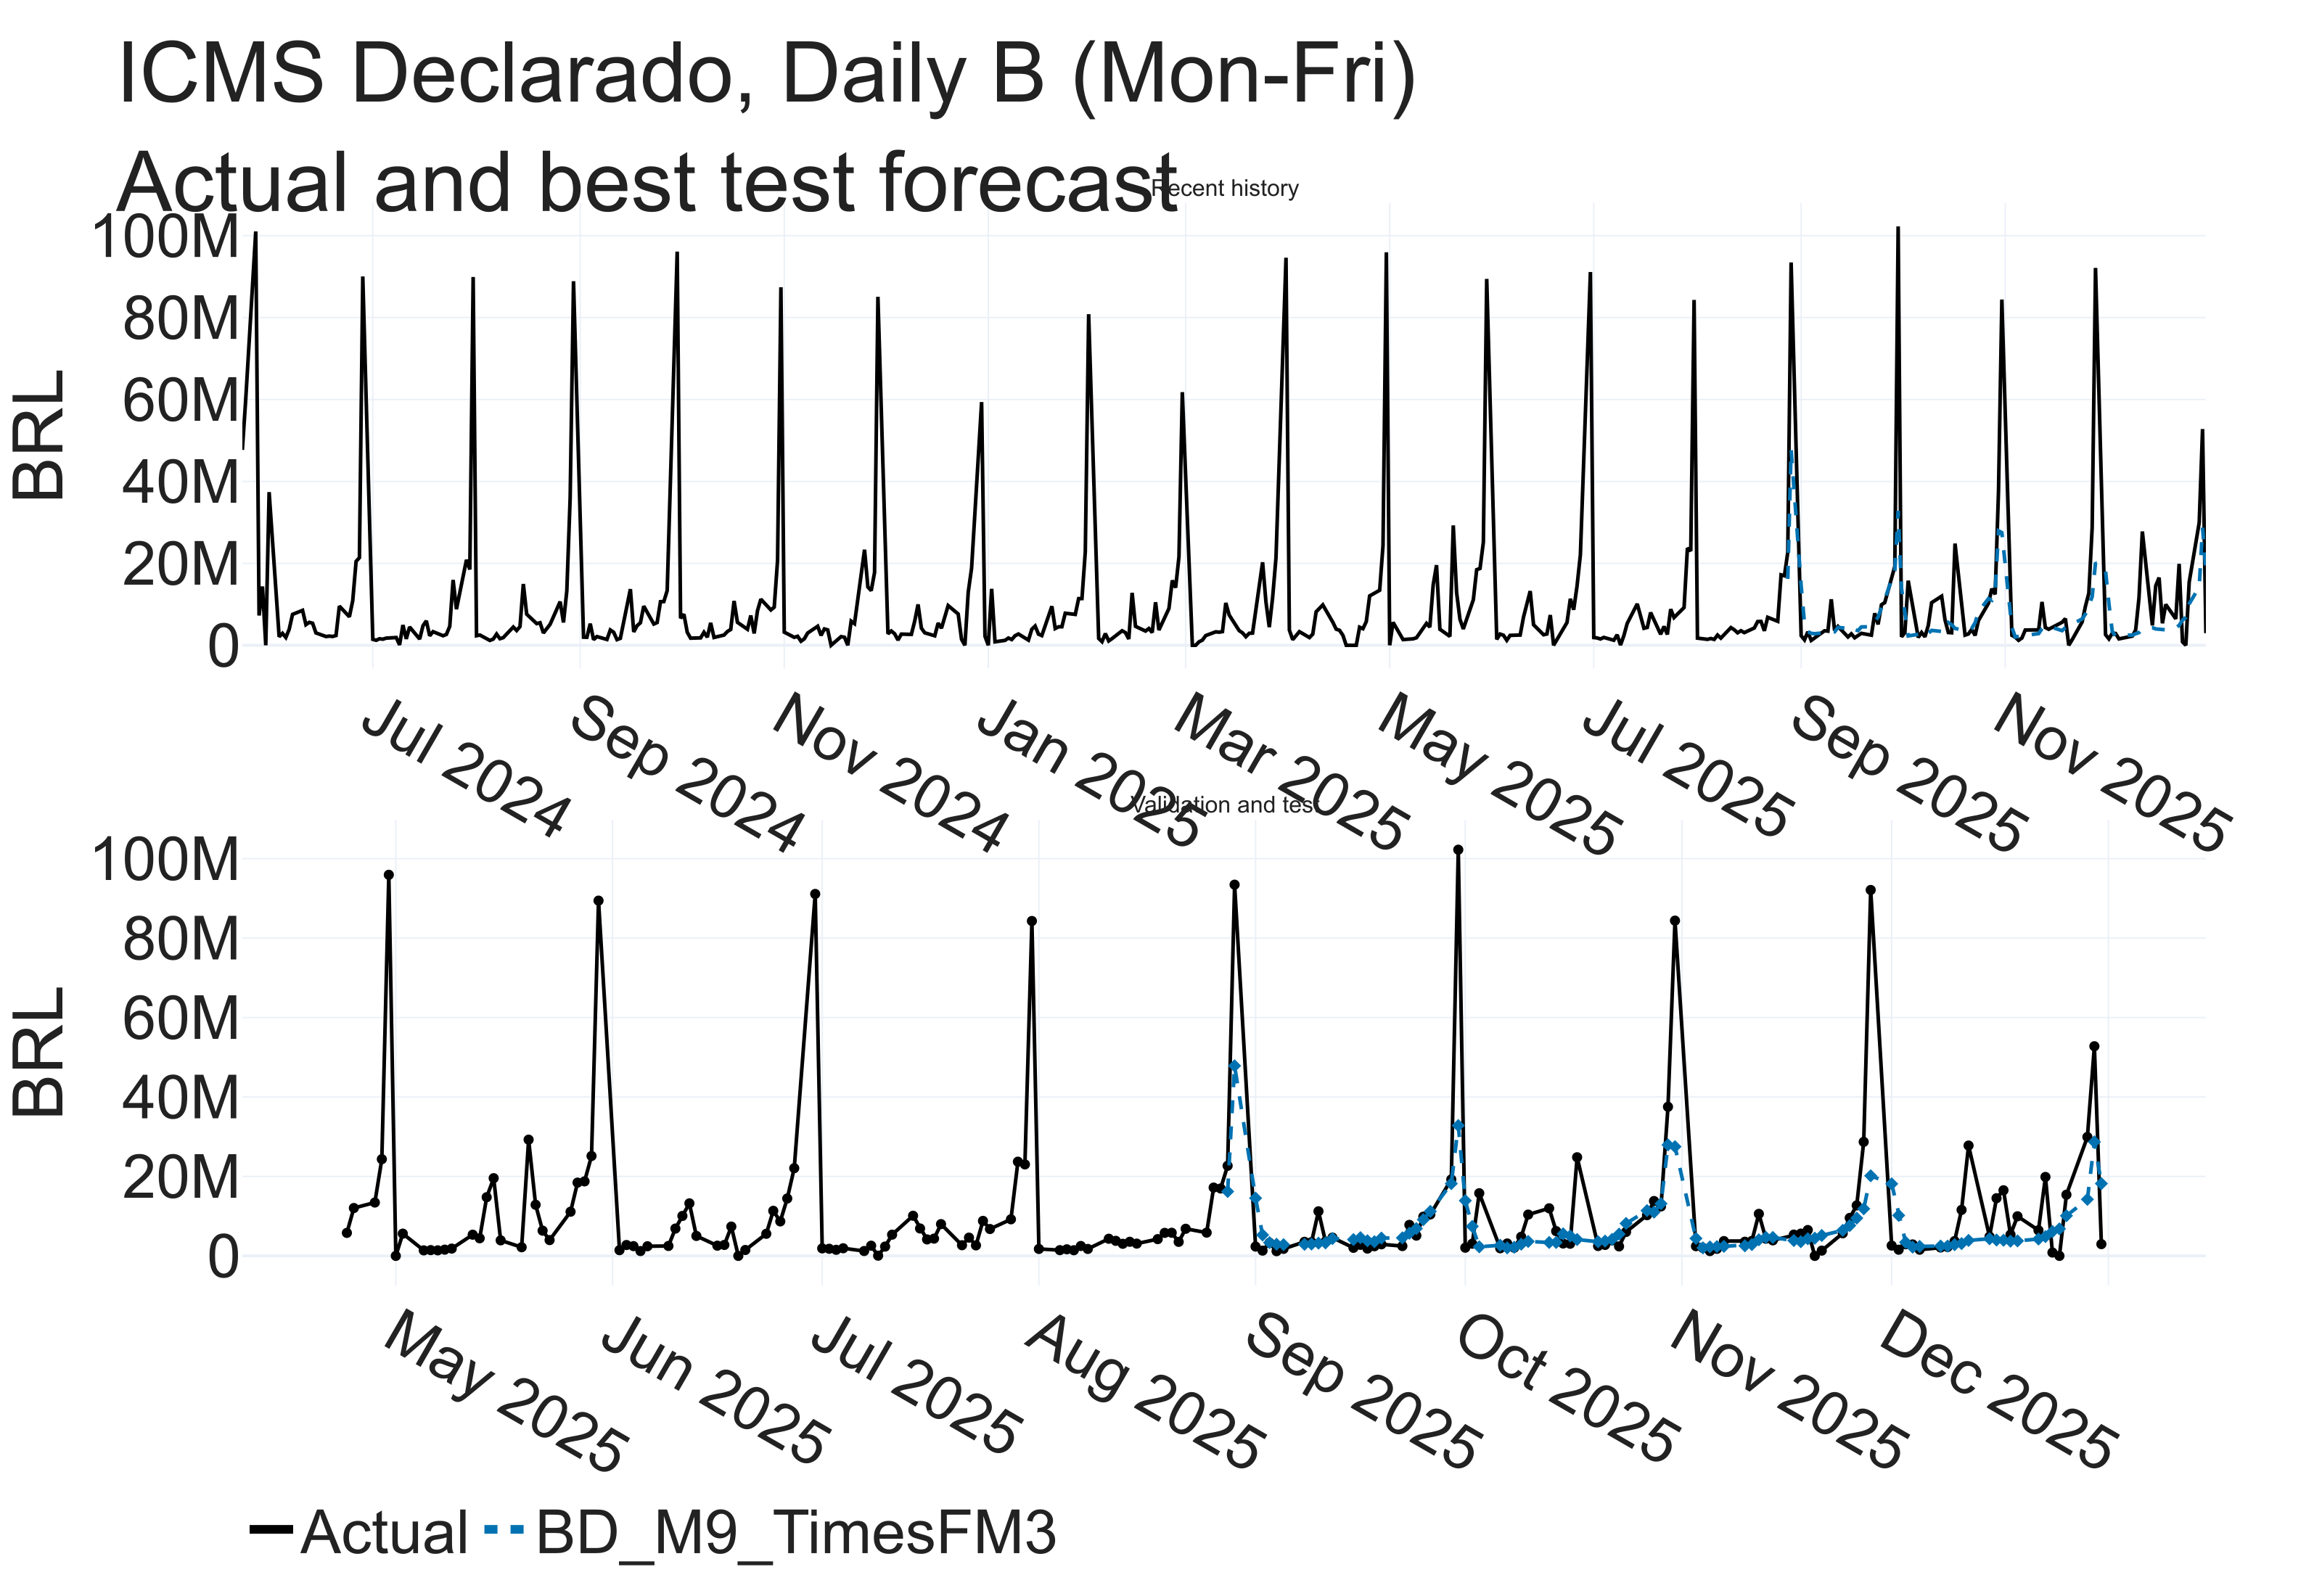
\includegraphics[width=\linewidth]{figures/segment/declarado_business_daily_forecast.png}
  \caption{Declarado, daily B. Blue dashed: M9 TimesFM.}
\end{figure}
\begin{figure}[H]
  \centering
  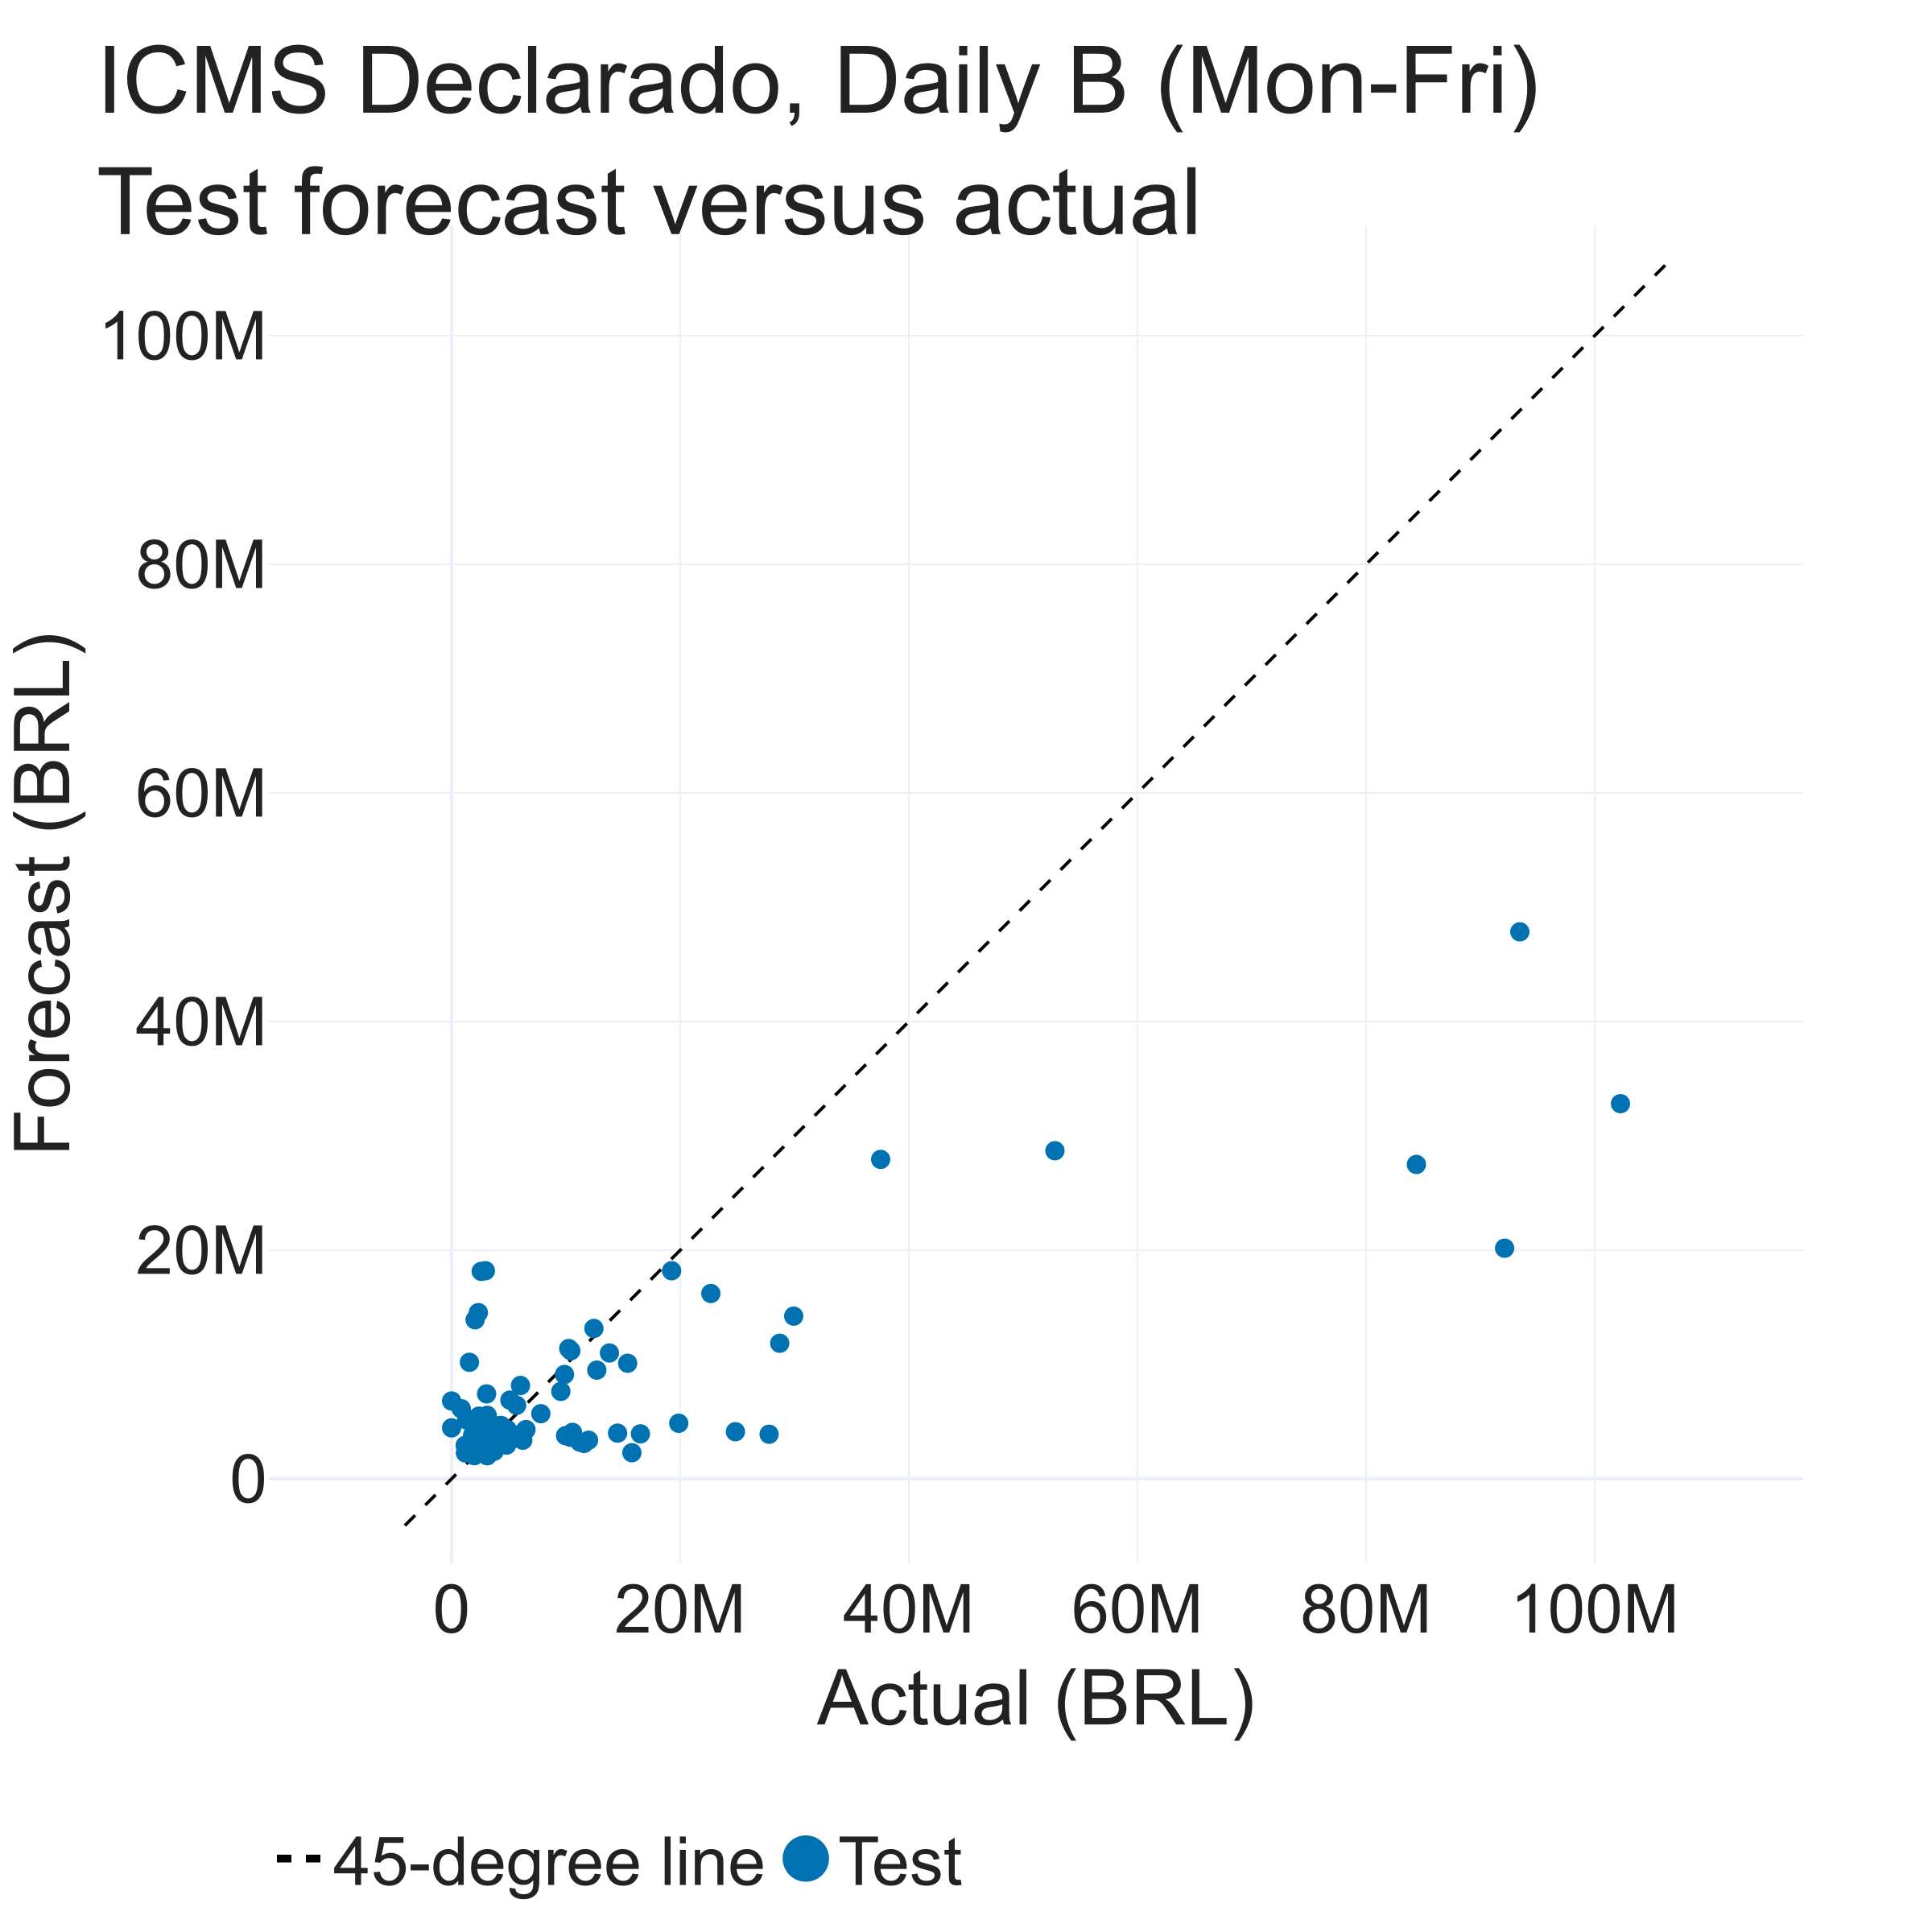
\includegraphics[width=0.62\linewidth]{figures/segment/declarado_business_daily_scatter.png}
  \caption{Declarado, daily B test scatter.}
\end{figure}
\begin{figure}[H]
  \centering
  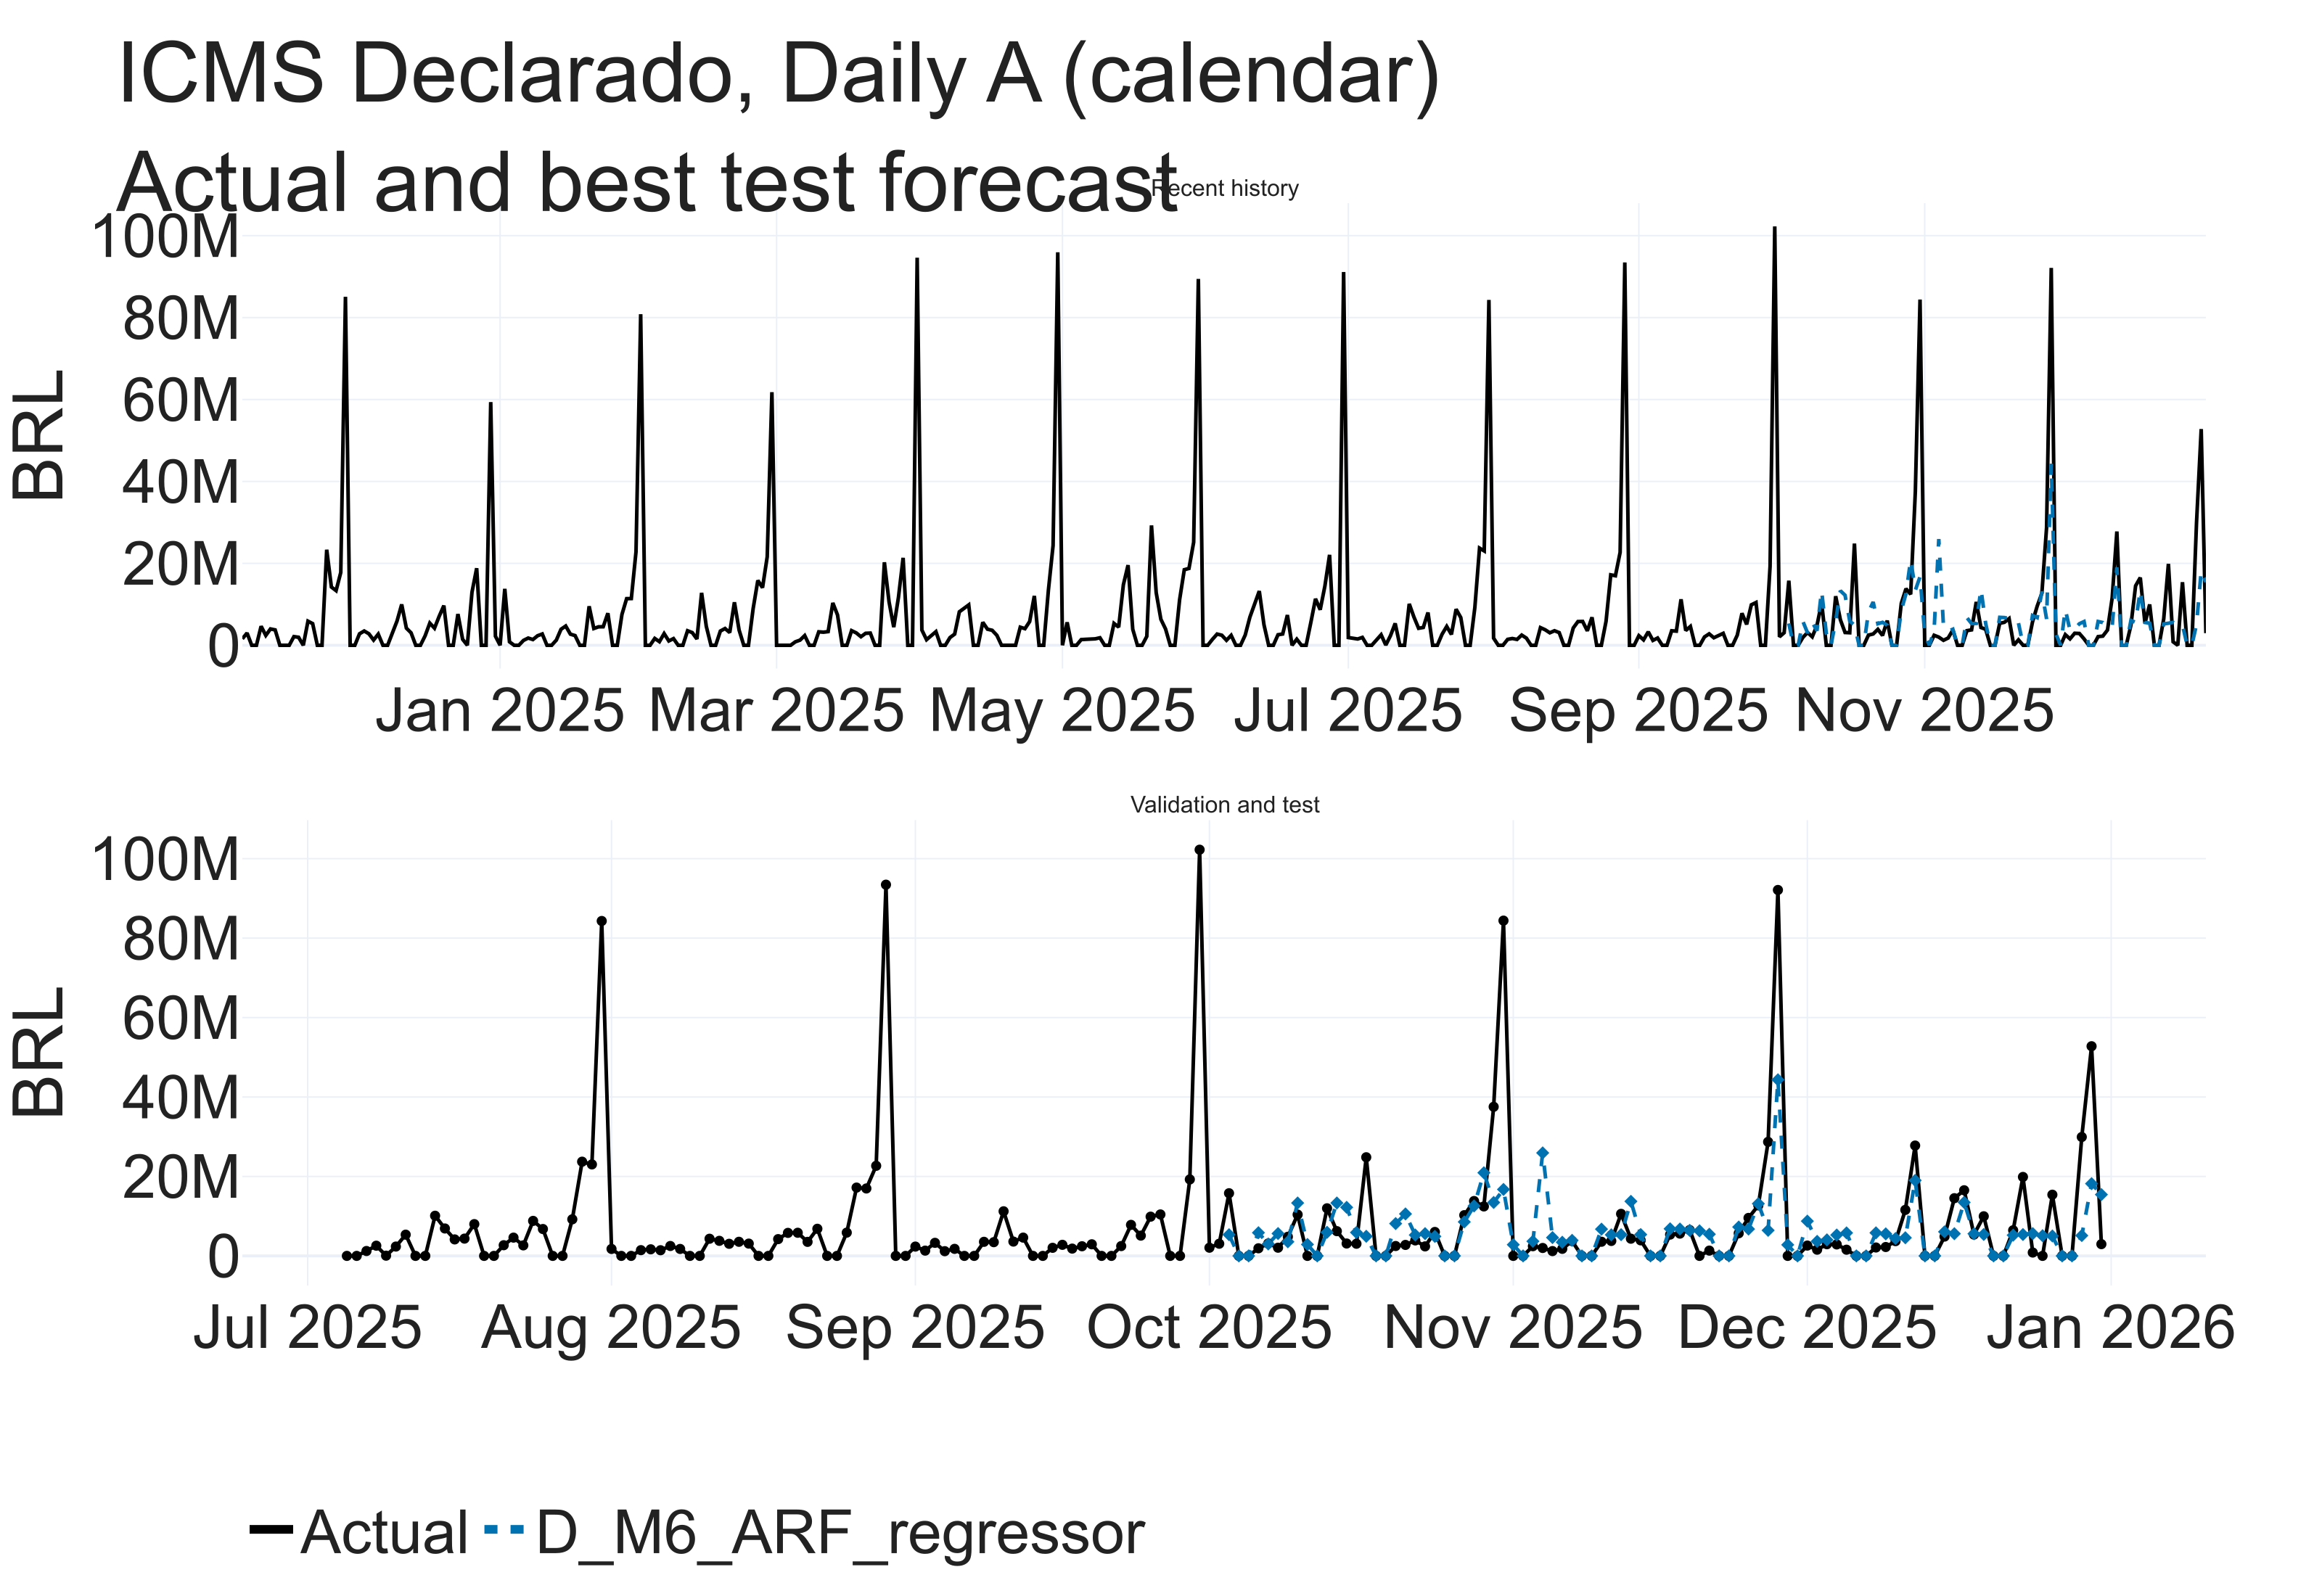
\includegraphics[width=\linewidth]{figures/segment/declarado_daily_forecast.png}
  \caption{Declarado, daily A. Blue dashed: M6 forest.}
\end{figure}
\begin{figure}[H]
  \centering
  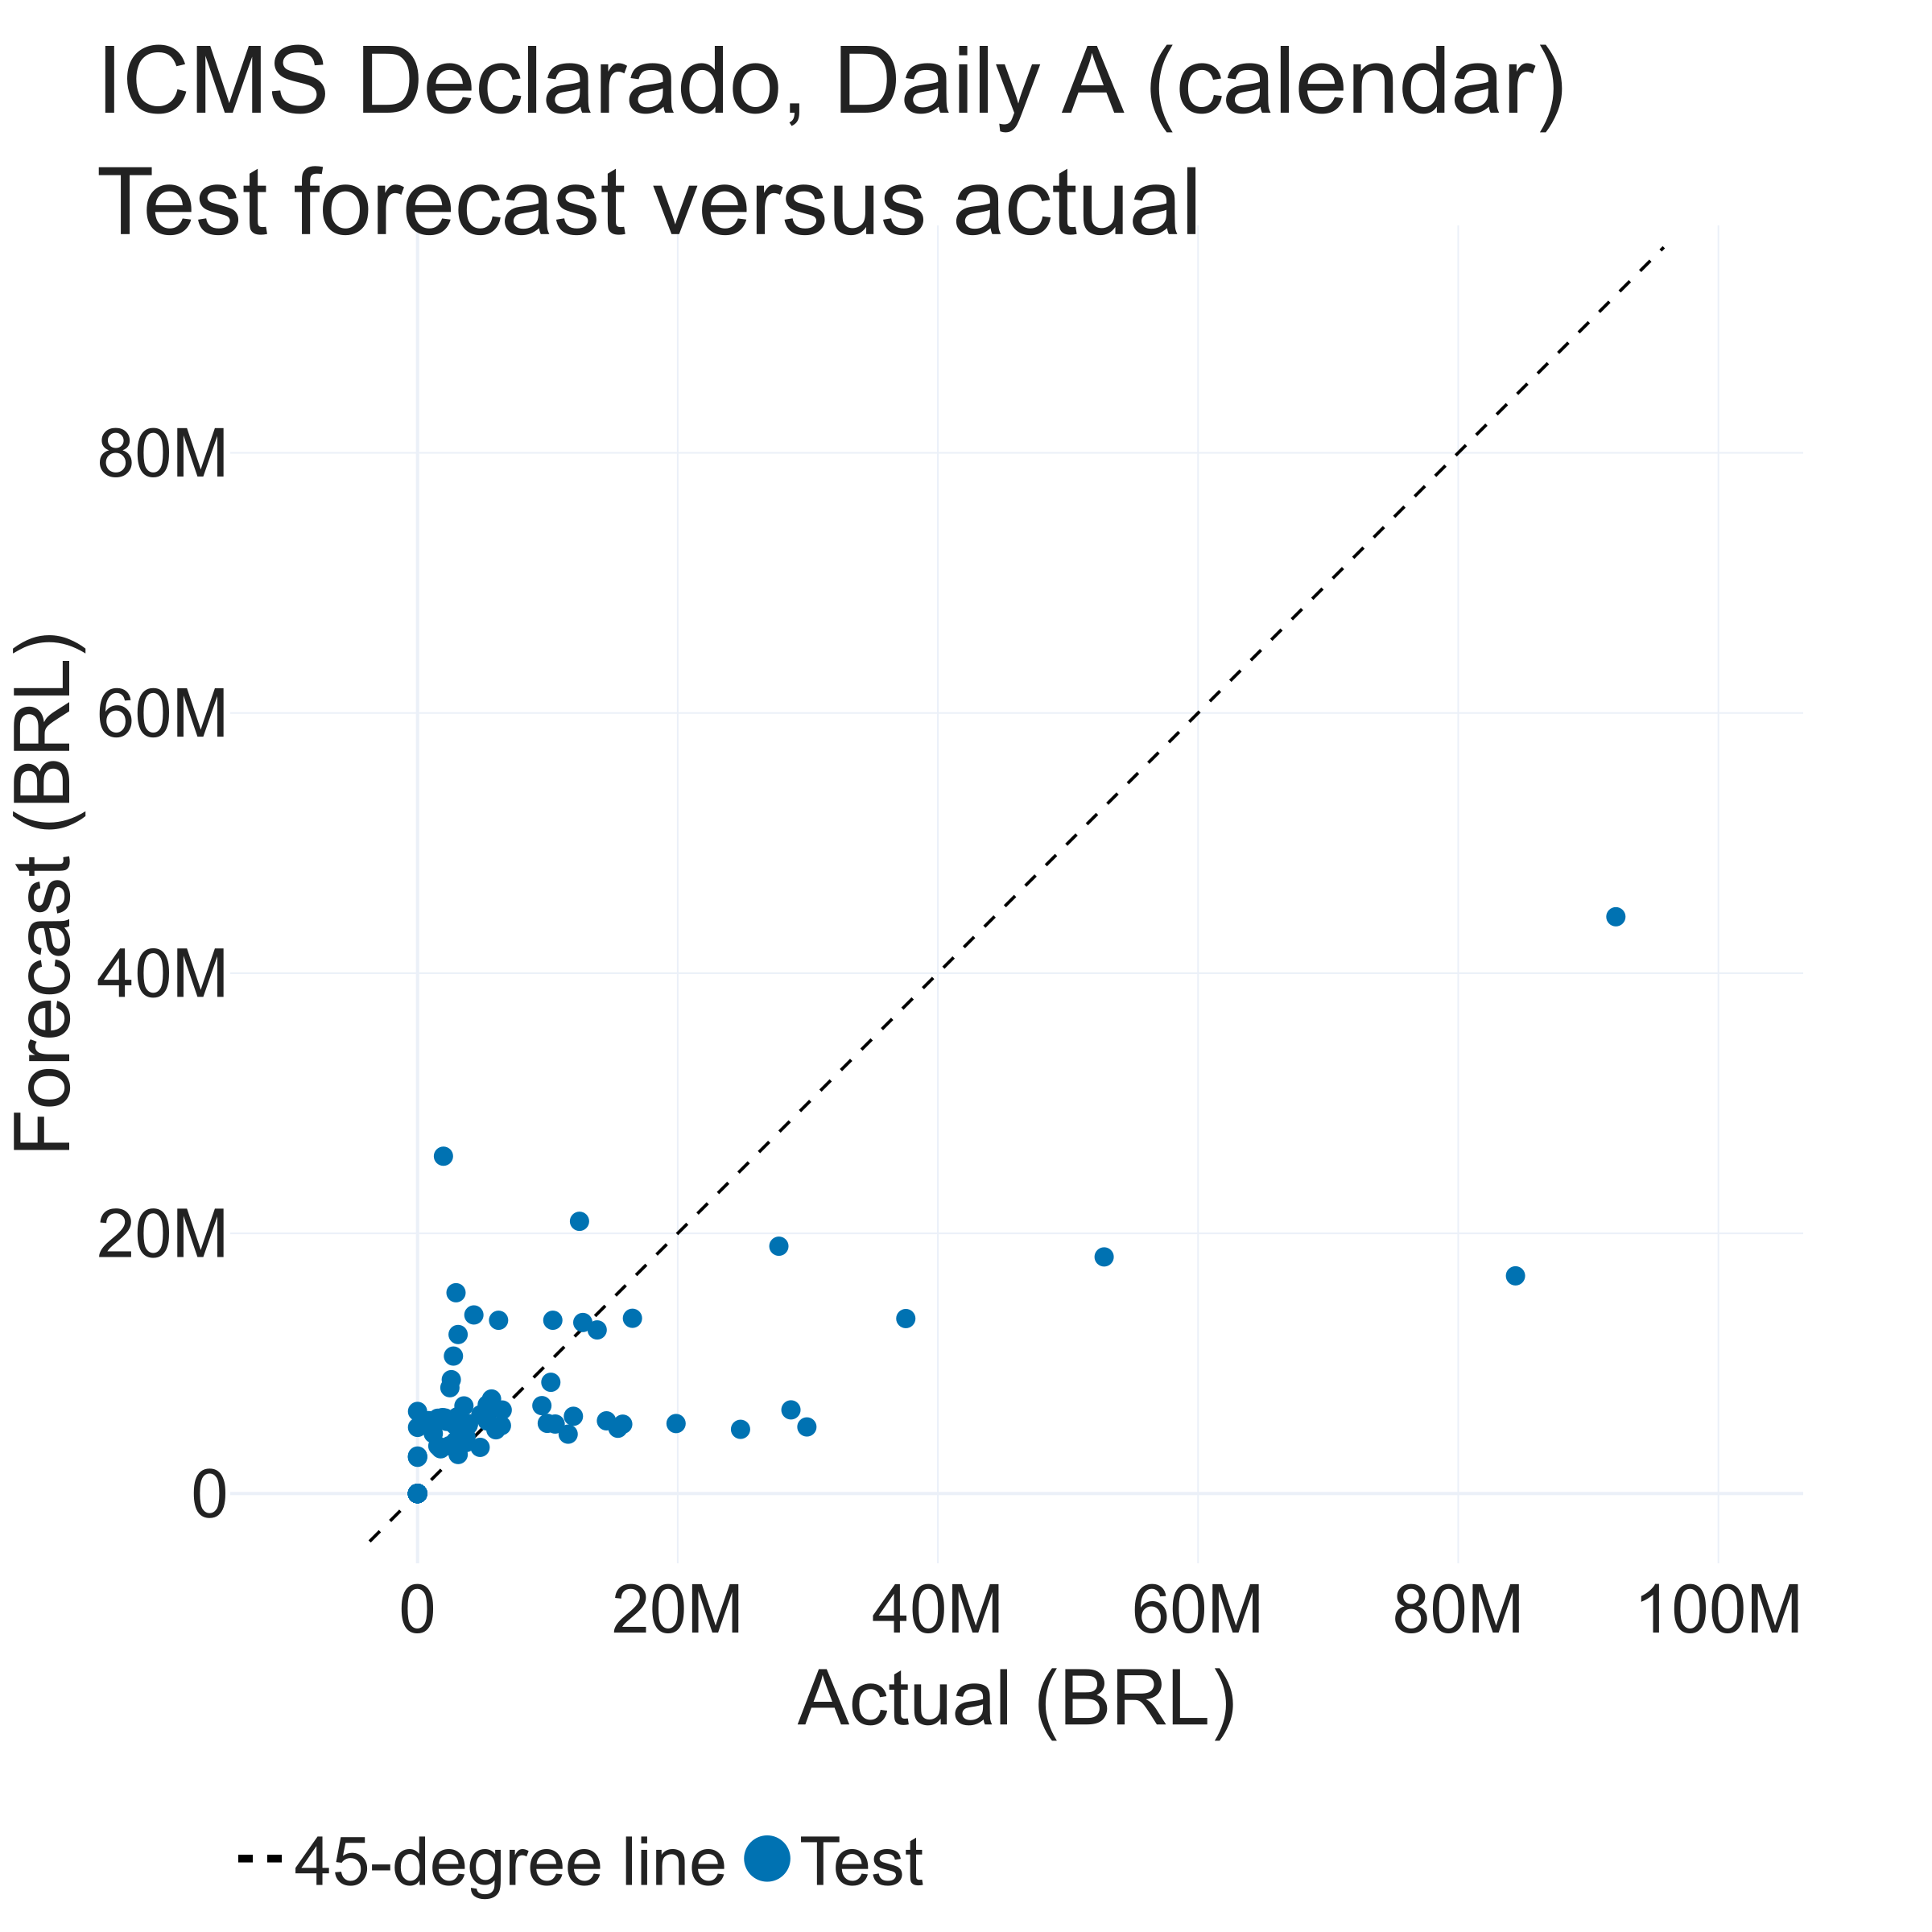
\includegraphics[width=0.62\linewidth]{figures/segment/declarado_daily_scatter.png}
  \caption{Declarado, daily A test scatter.}
\end{figure}
\begin{figure}[H]
  \centering
  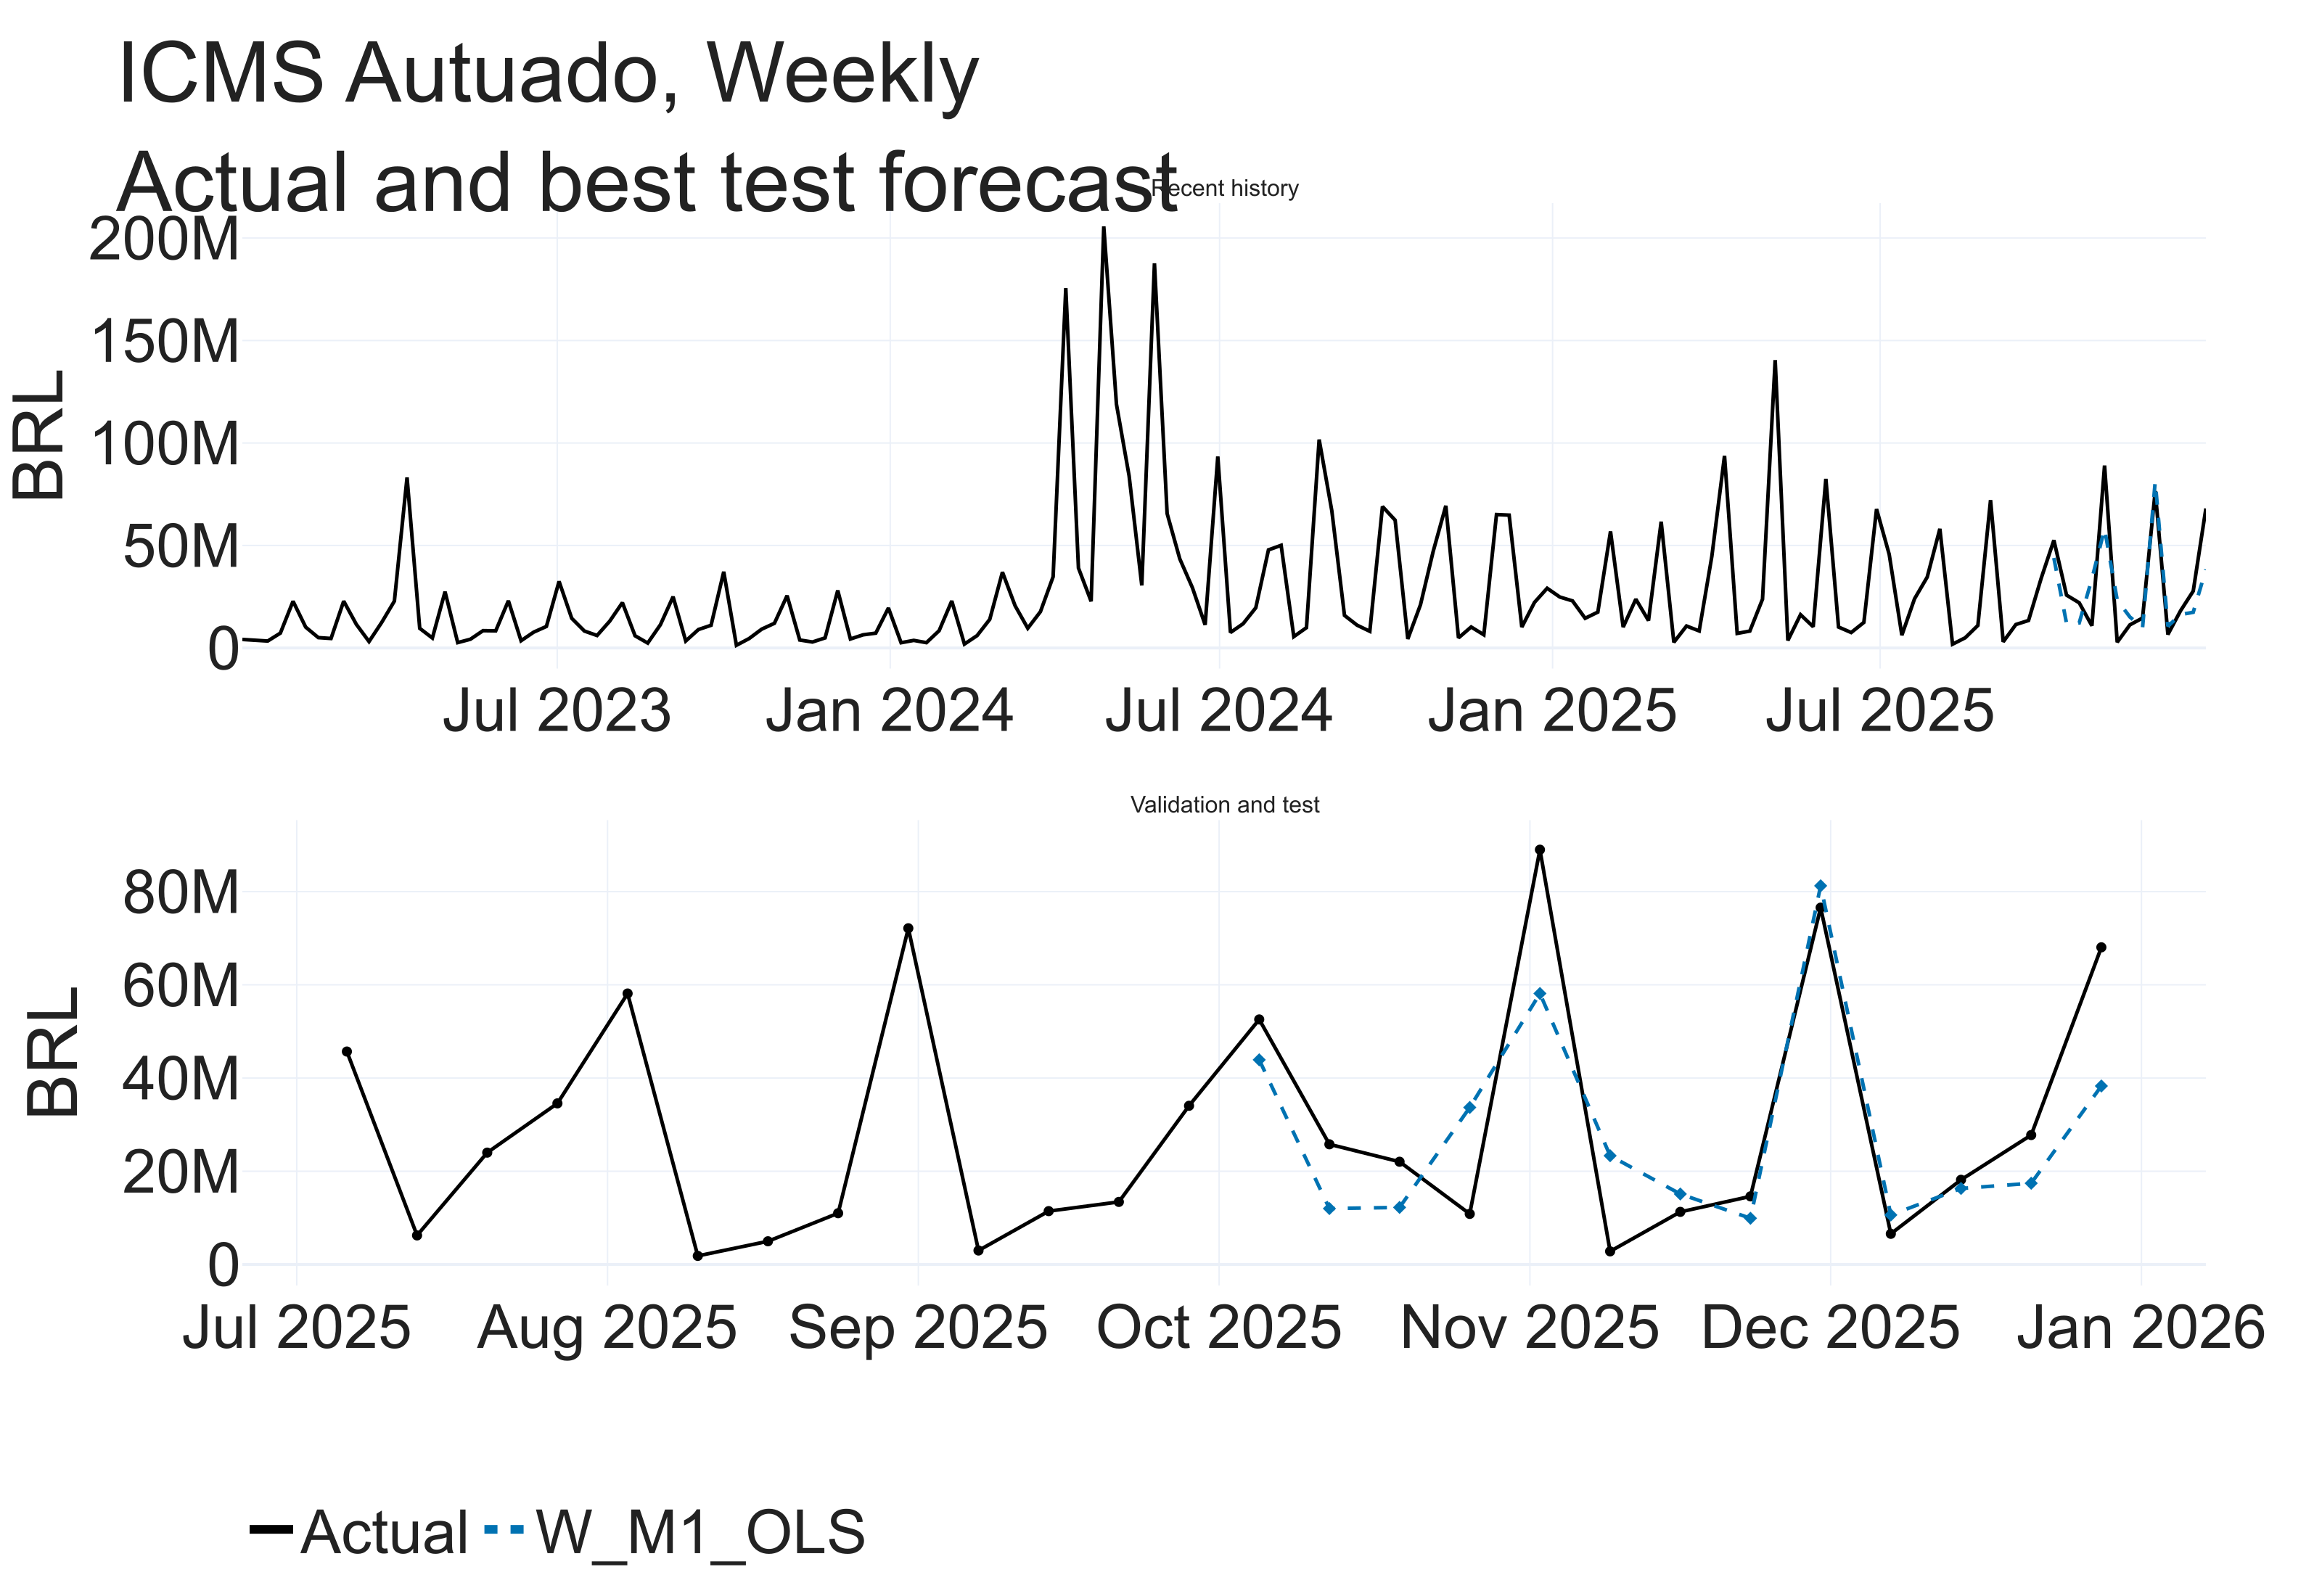
\includegraphics[width=\linewidth]{figures/segment/autuado_weekly_forecast.png}
  \caption{Autuado, weekly. Blue dashed: M1 least squares.}
\end{figure}
\begin{figure}[H]
  \centering
  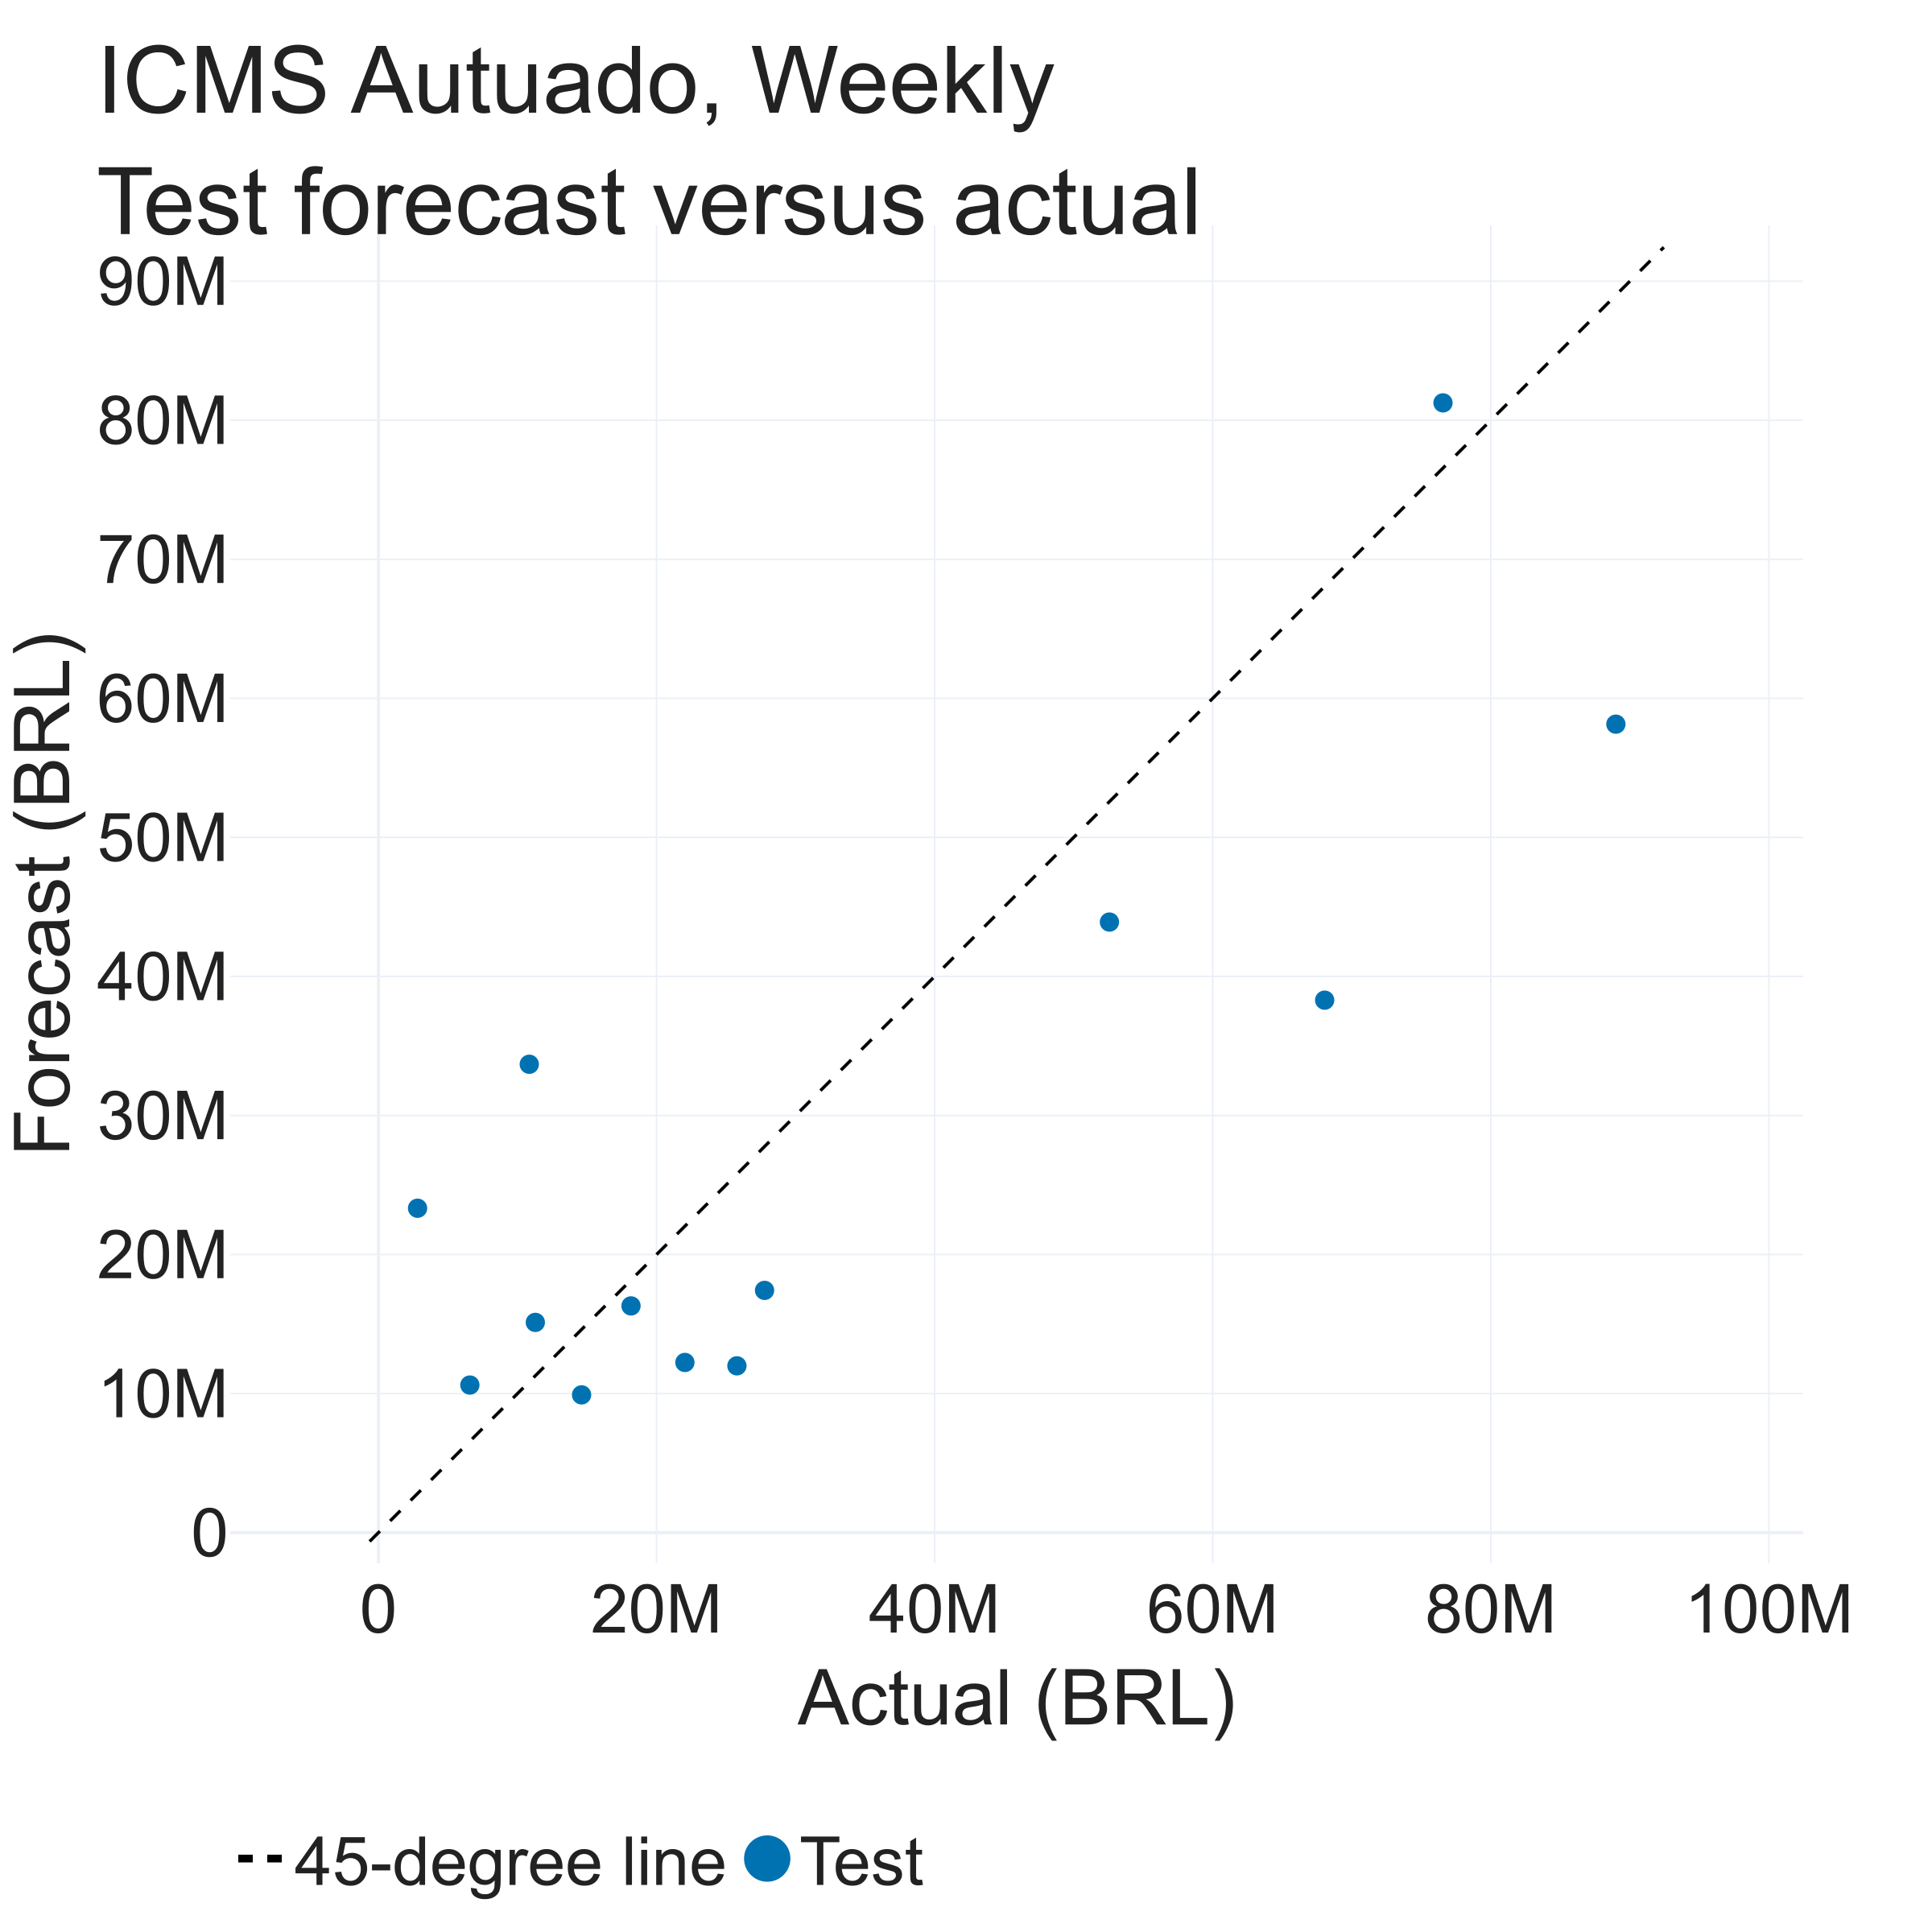
\includegraphics[width=0.62\linewidth]{figures/segment/autuado_weekly_scatter.png}
  \caption{Autuado, weekly test scatter.}
\end{figure}
\begin{figure}[H]
  \centering
  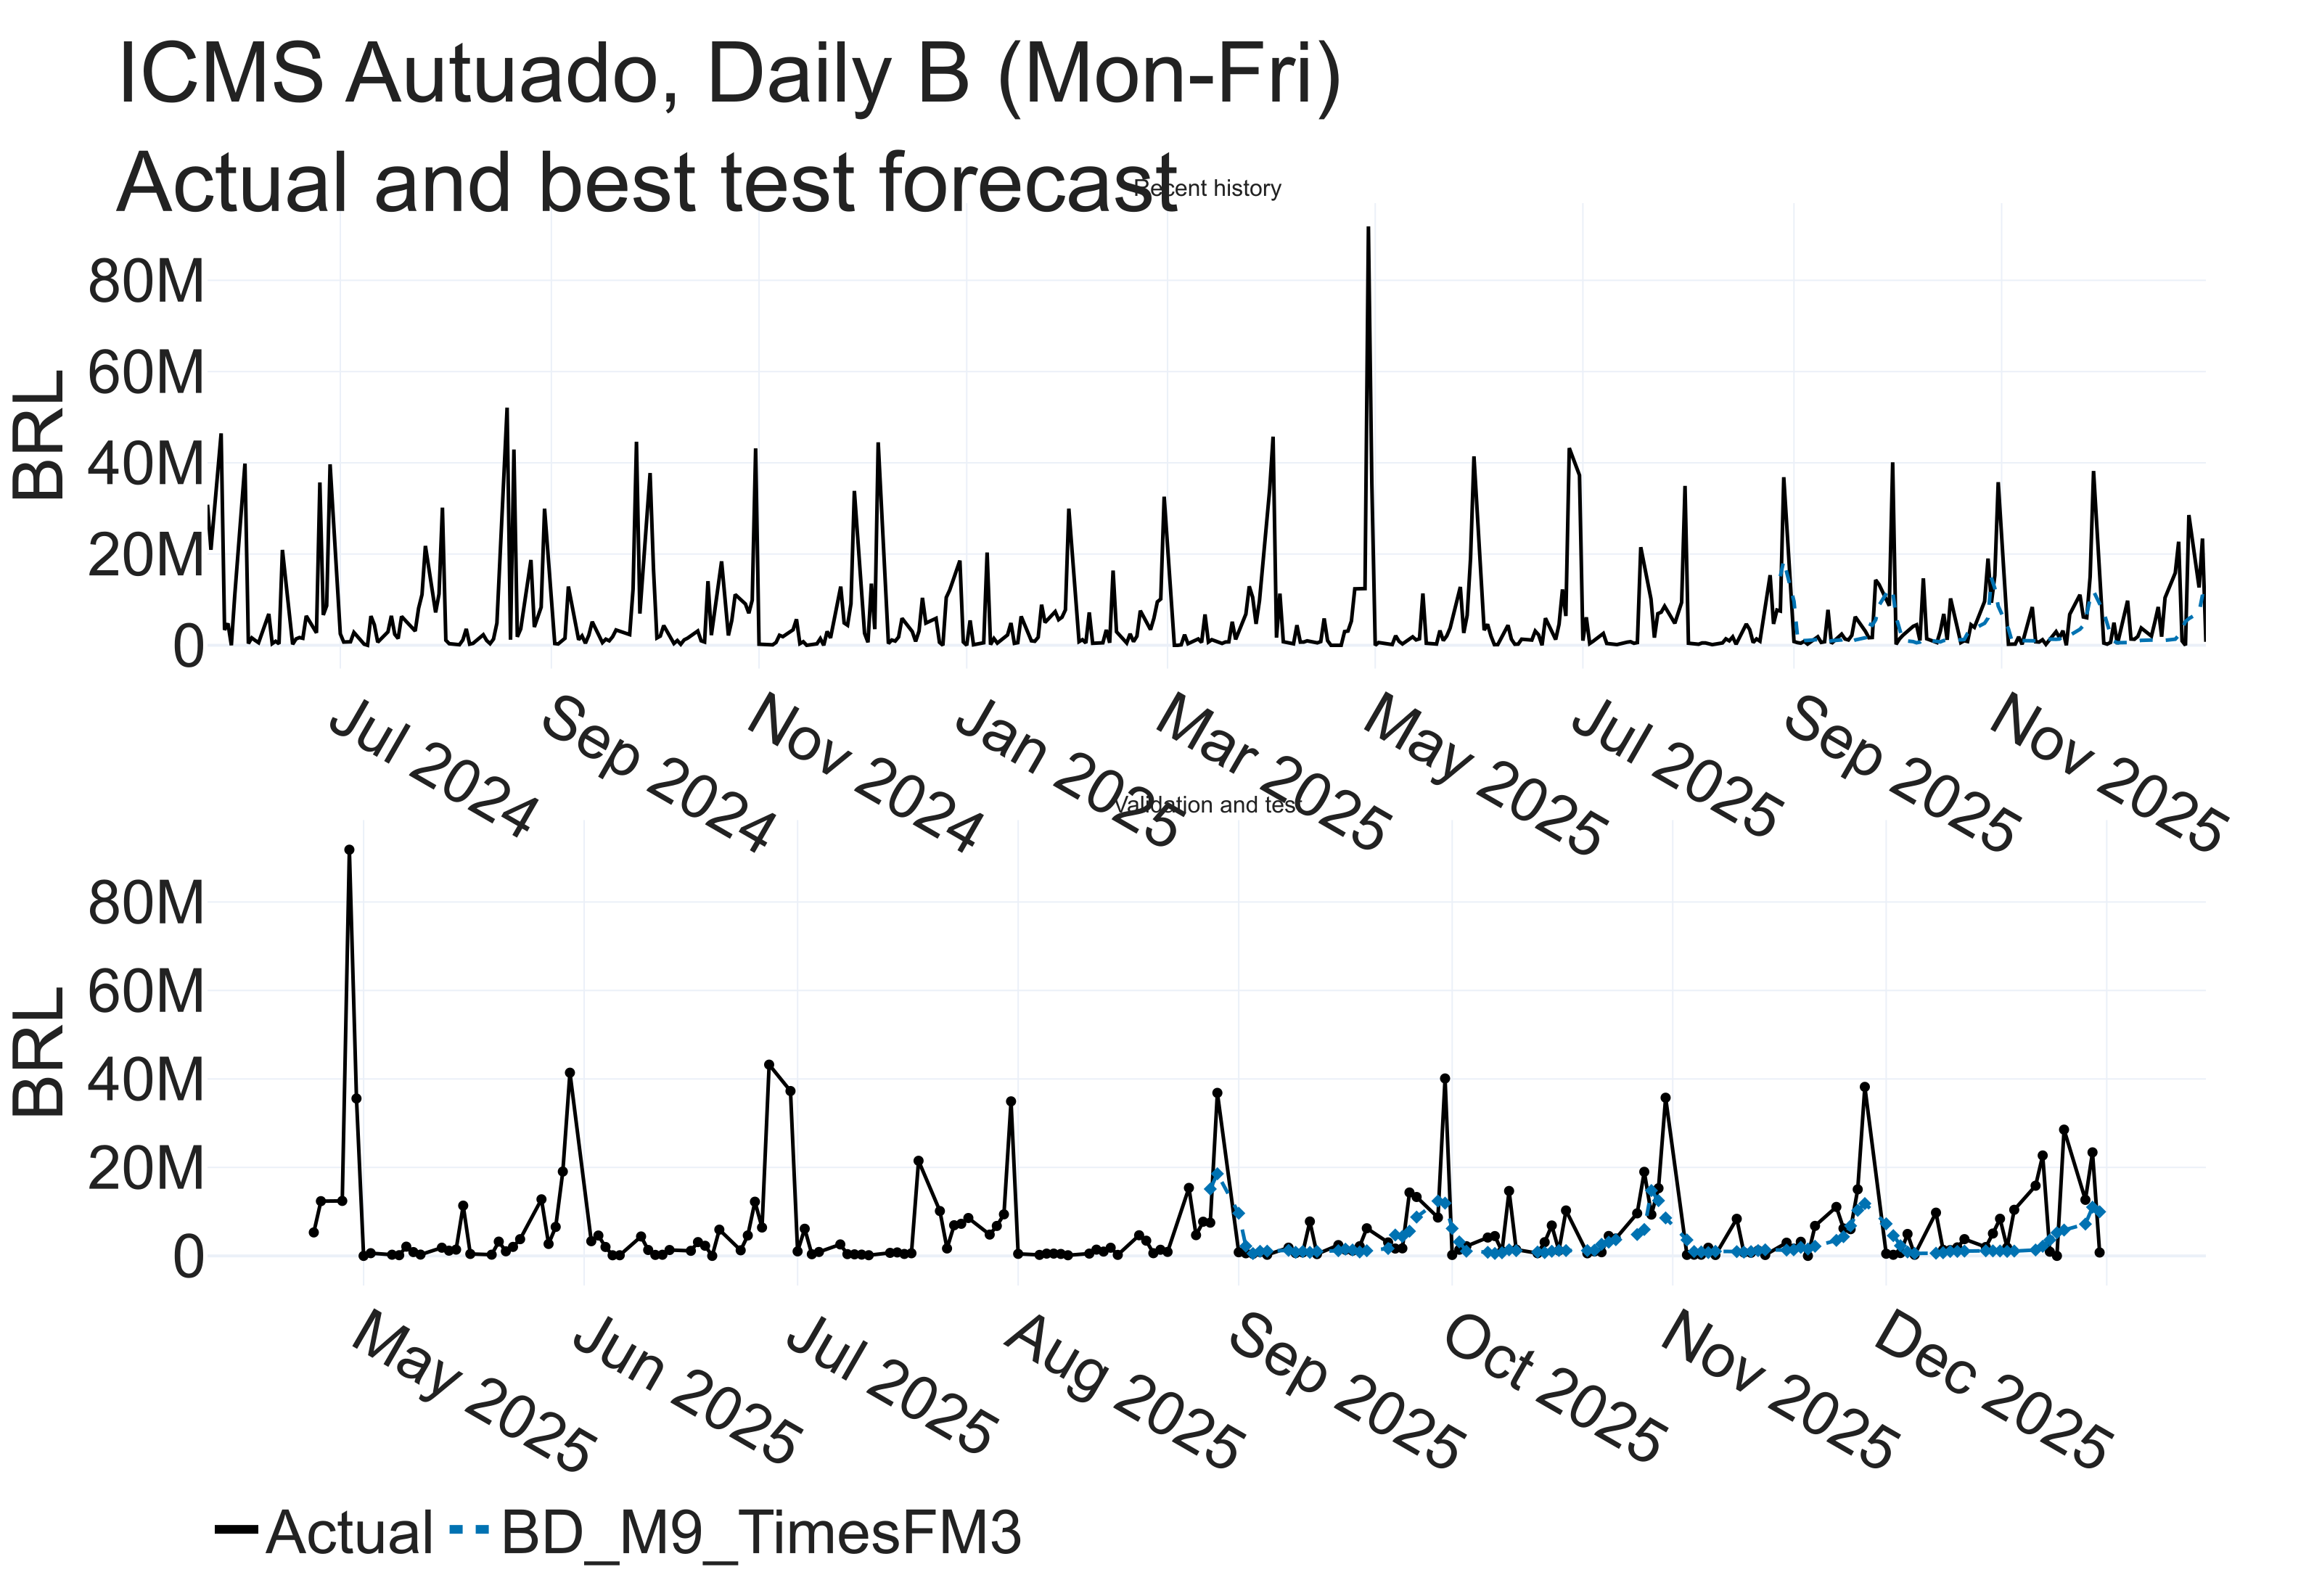
\includegraphics[width=\linewidth]{figures/segment/autuado_business_daily_forecast.png}
  \caption{Autuado, daily B. Blue dashed: M9 TimesFM.}
\end{figure}
\begin{figure}[H]
  \centering
  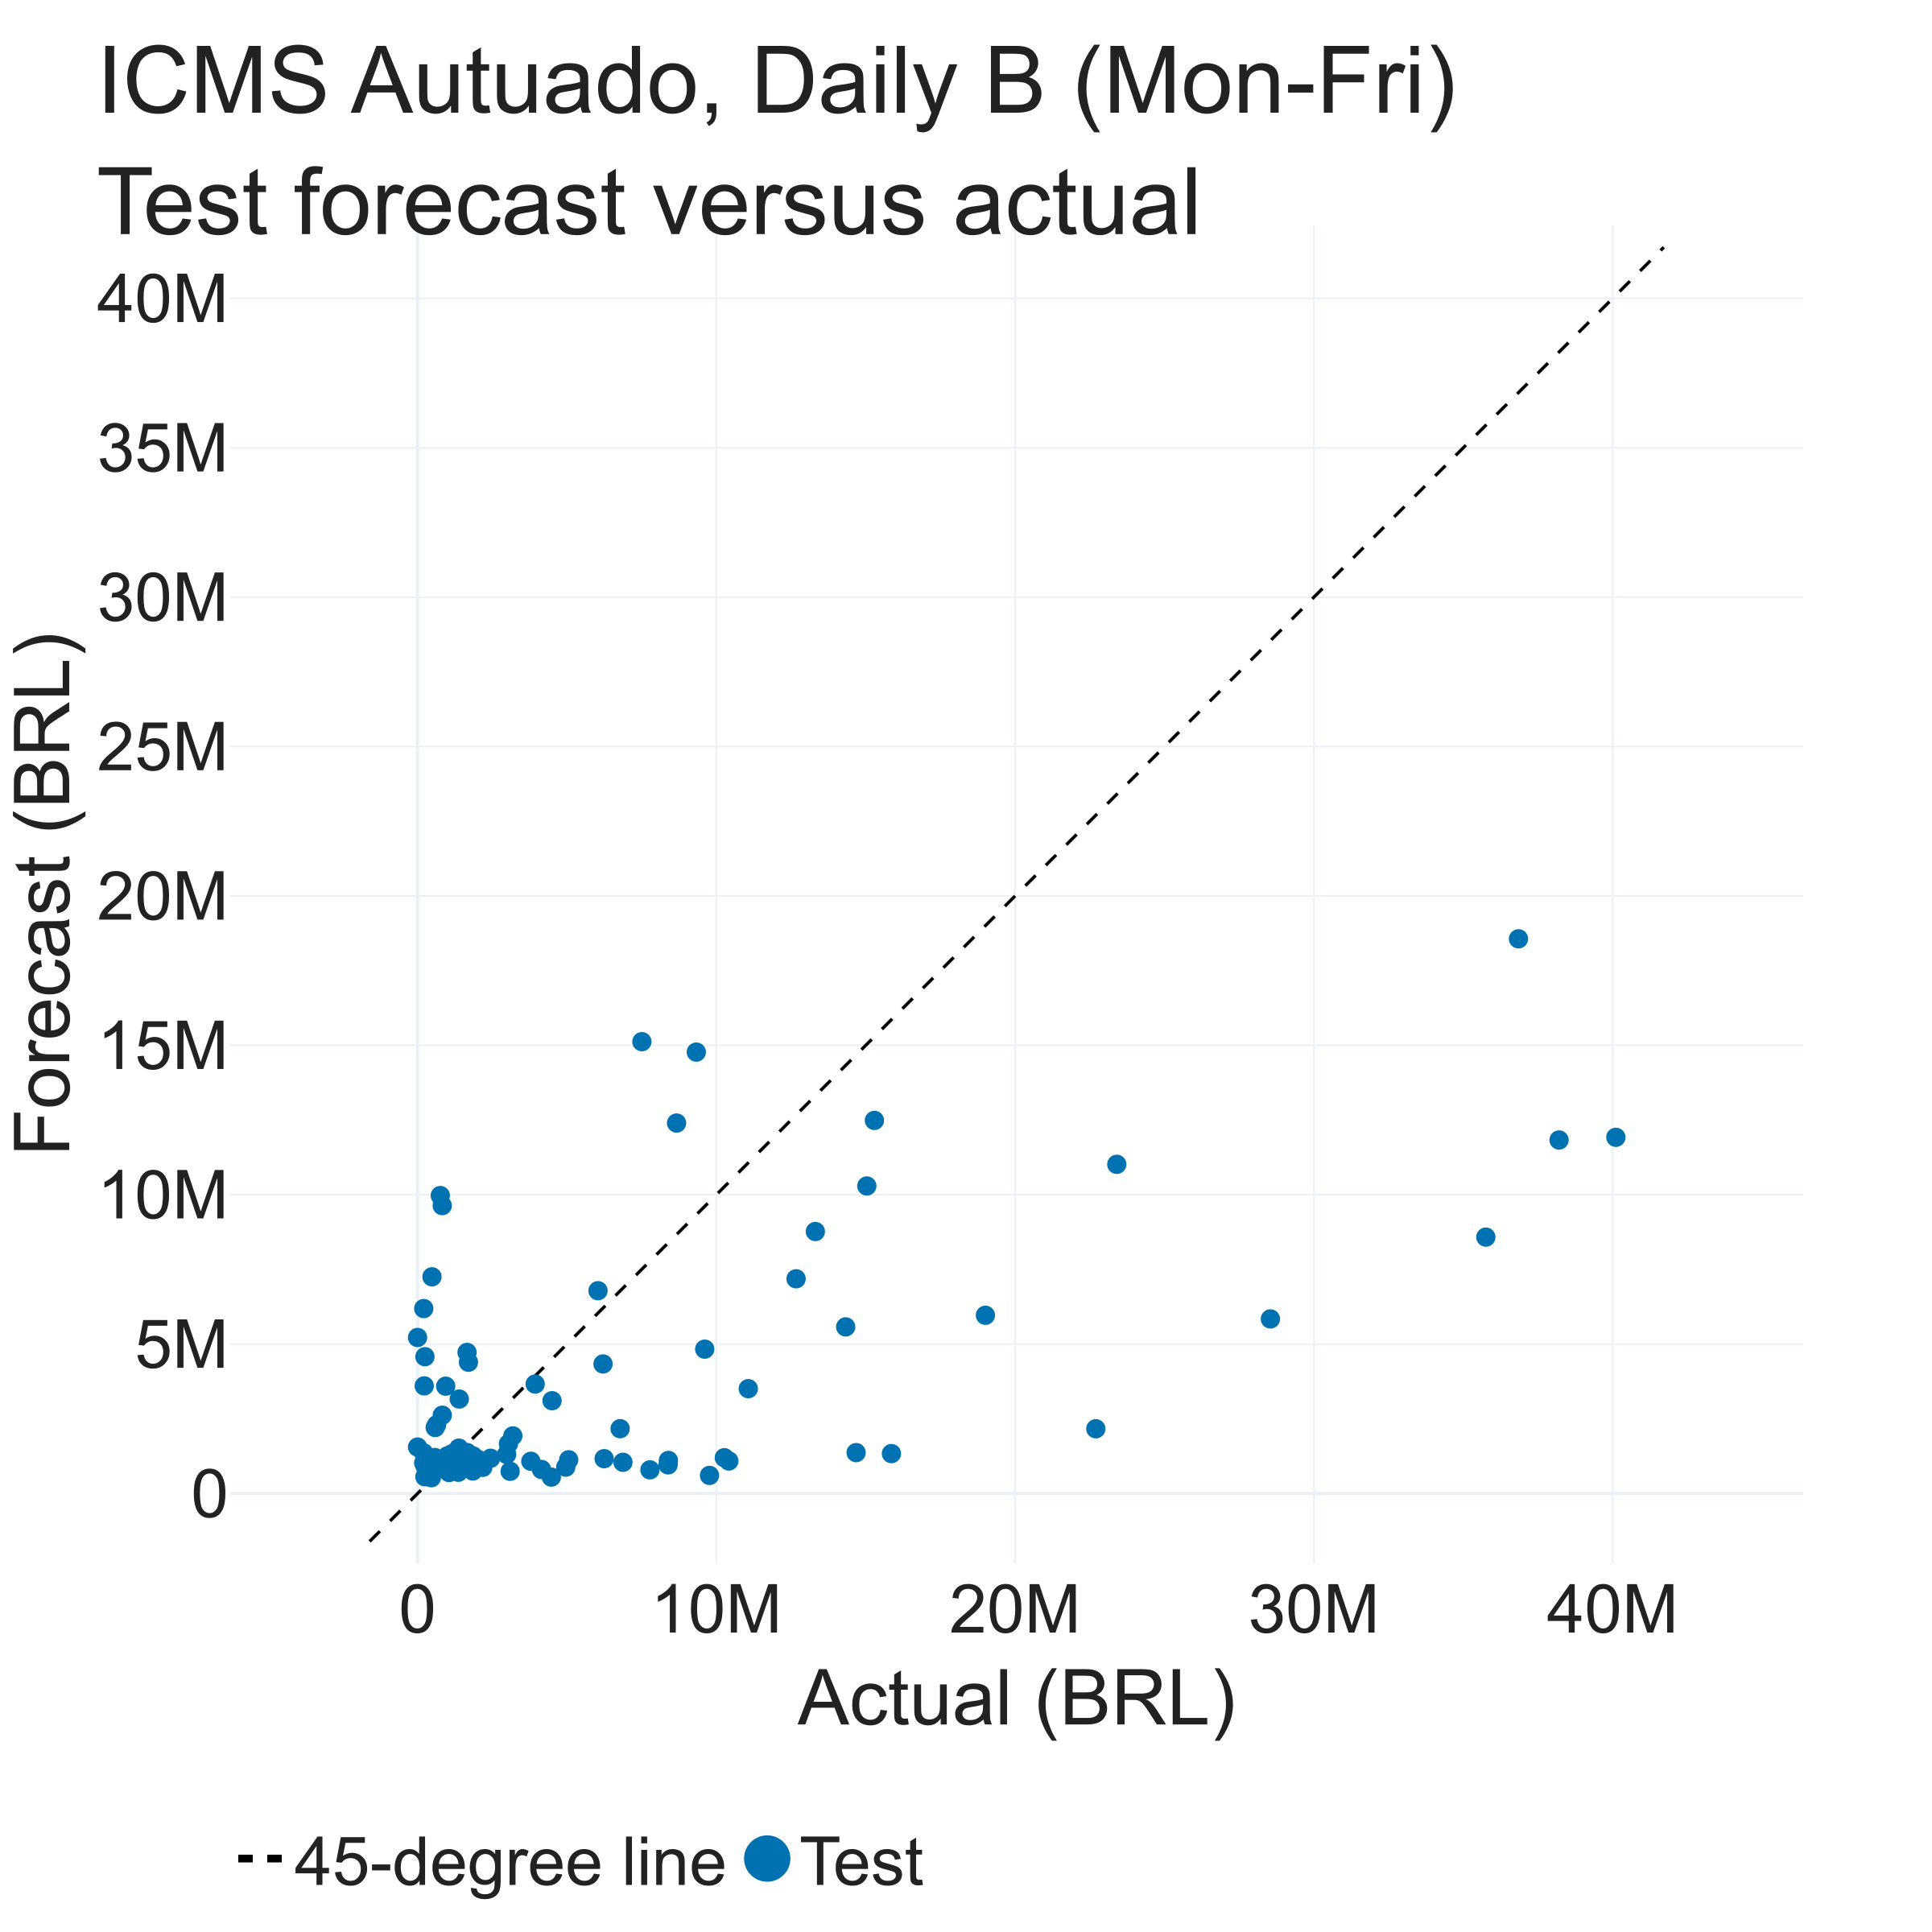
\includegraphics[width=0.62\linewidth]{figures/segment/autuado_business_daily_scatter.png}
  \caption{Autuado, daily B test scatter.}
\end{figure}
\begin{figure}[H]
  \centering
  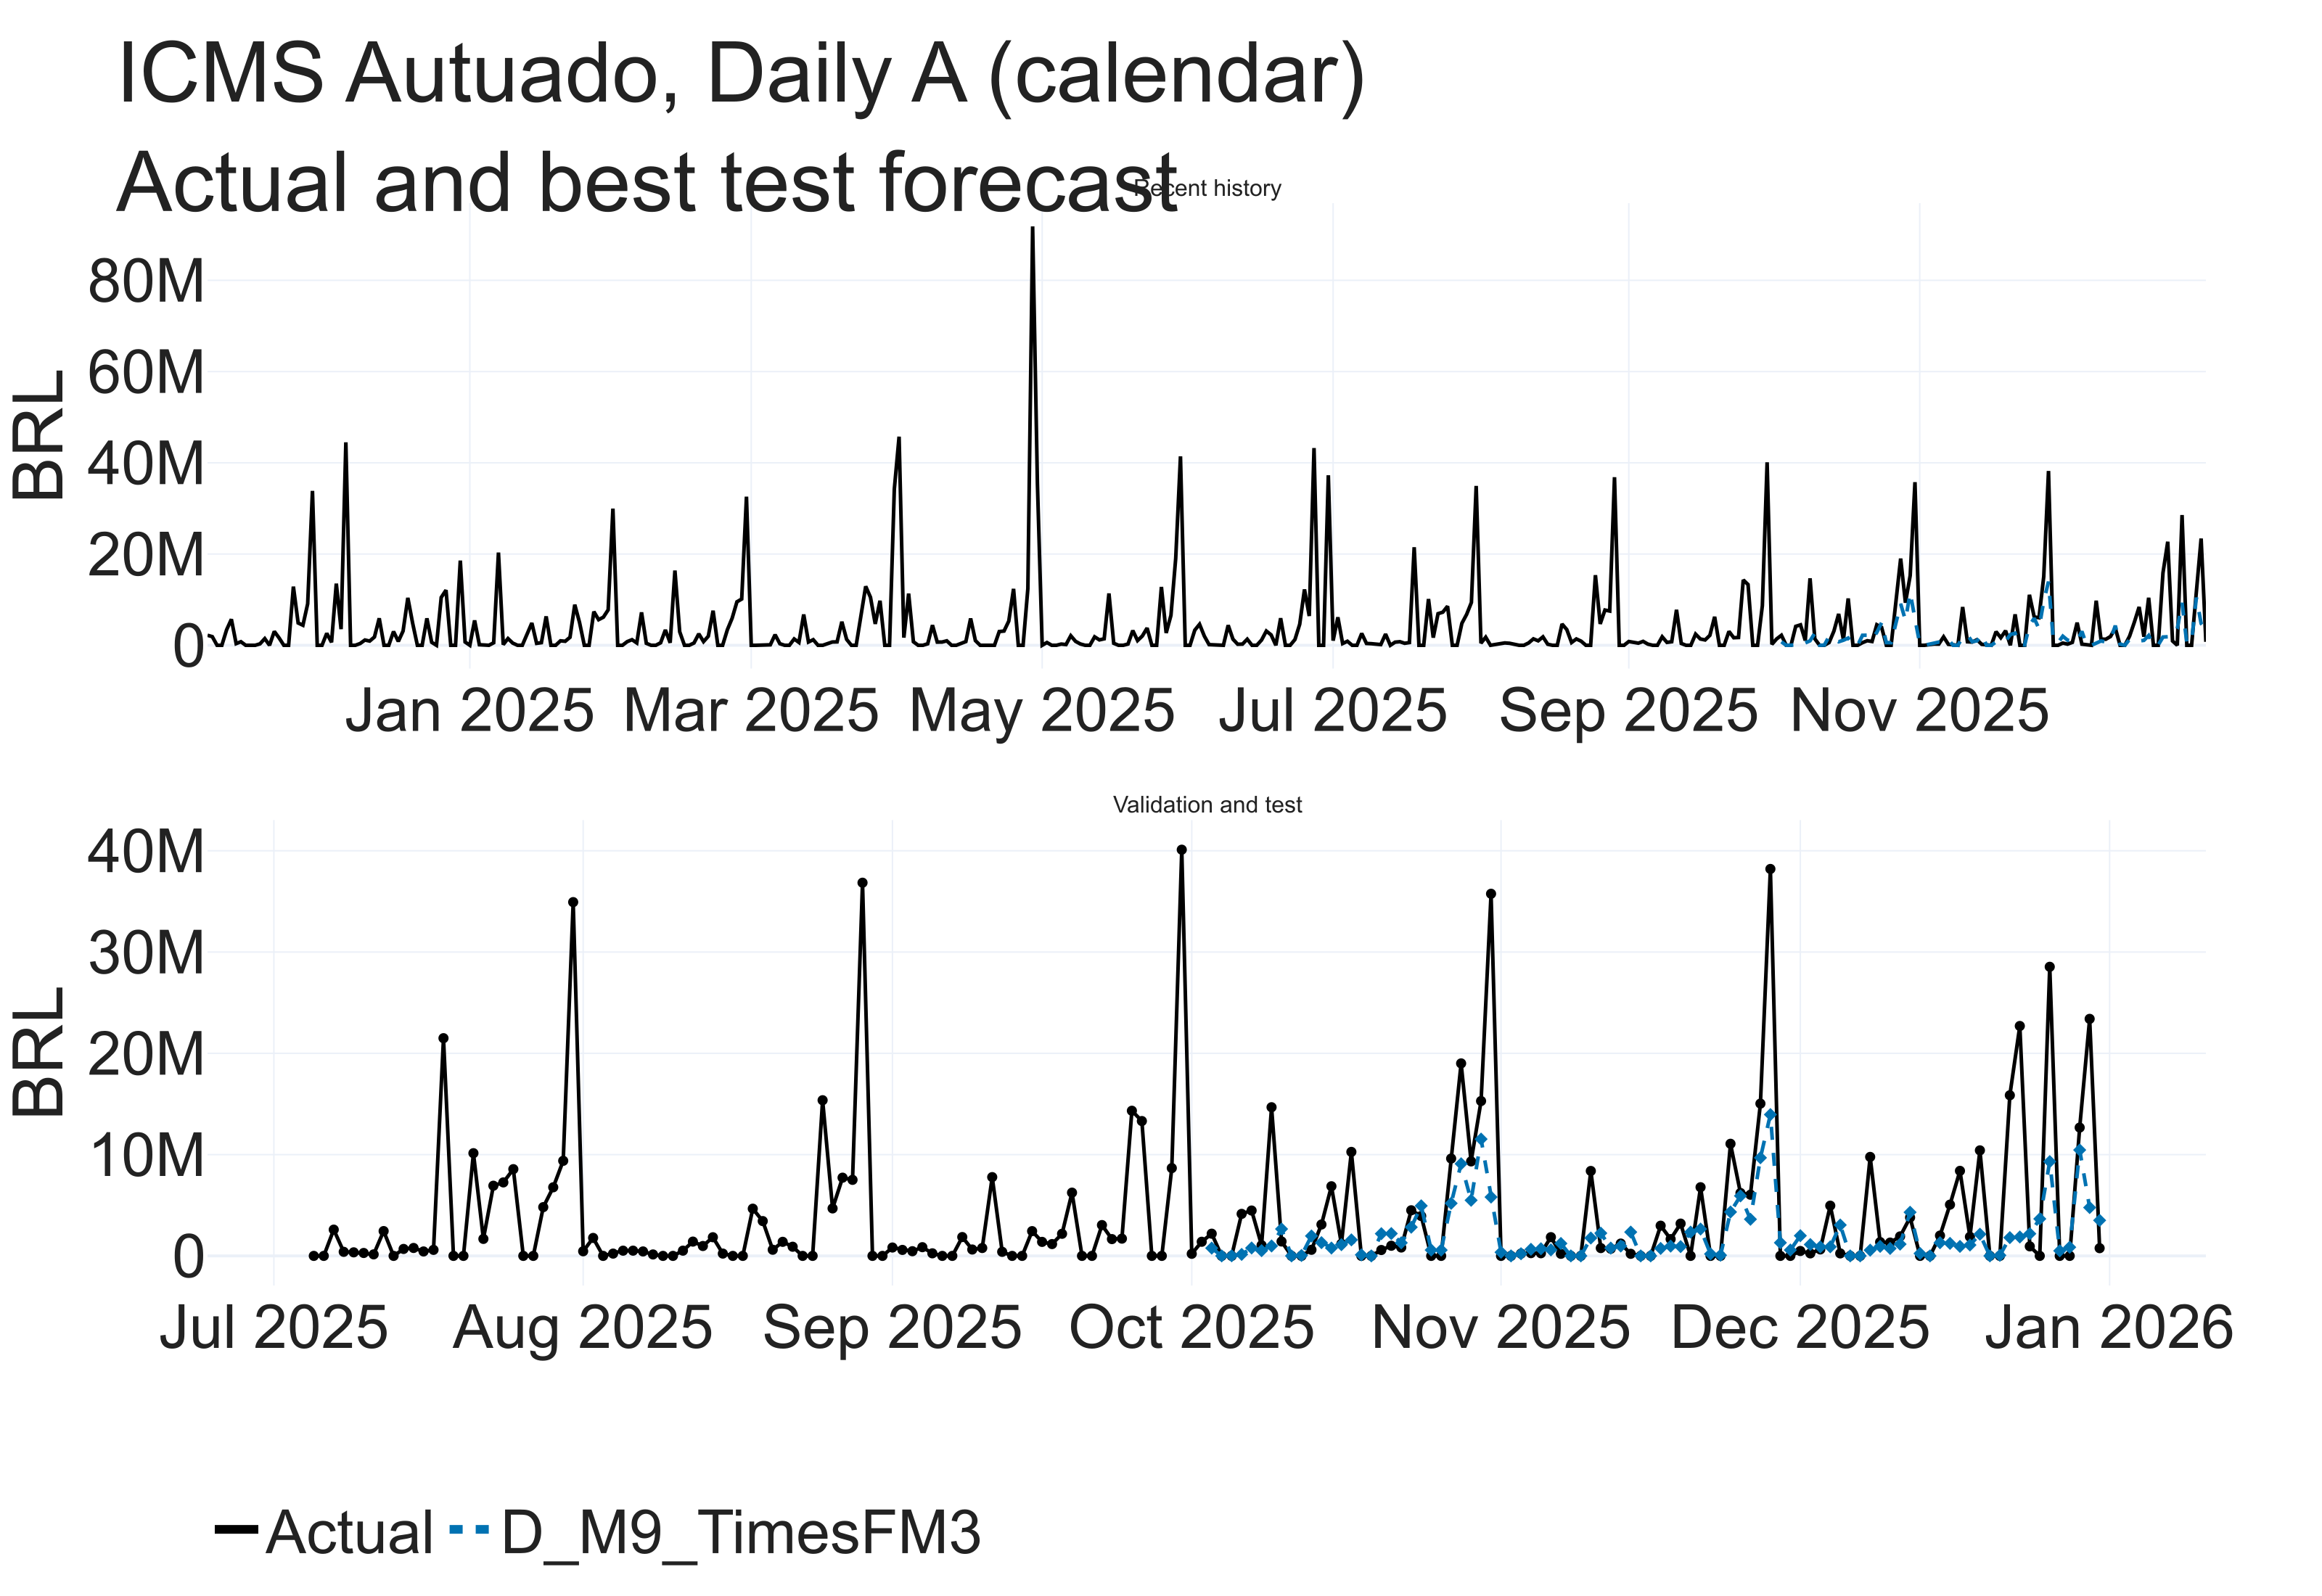
\includegraphics[width=\linewidth]{figures/segment/autuado_daily_forecast.png}
  \caption{Autuado, daily A. Blue dashed: M9 TimesFM.}
\end{figure}
\begin{figure}[H]
  \centering
  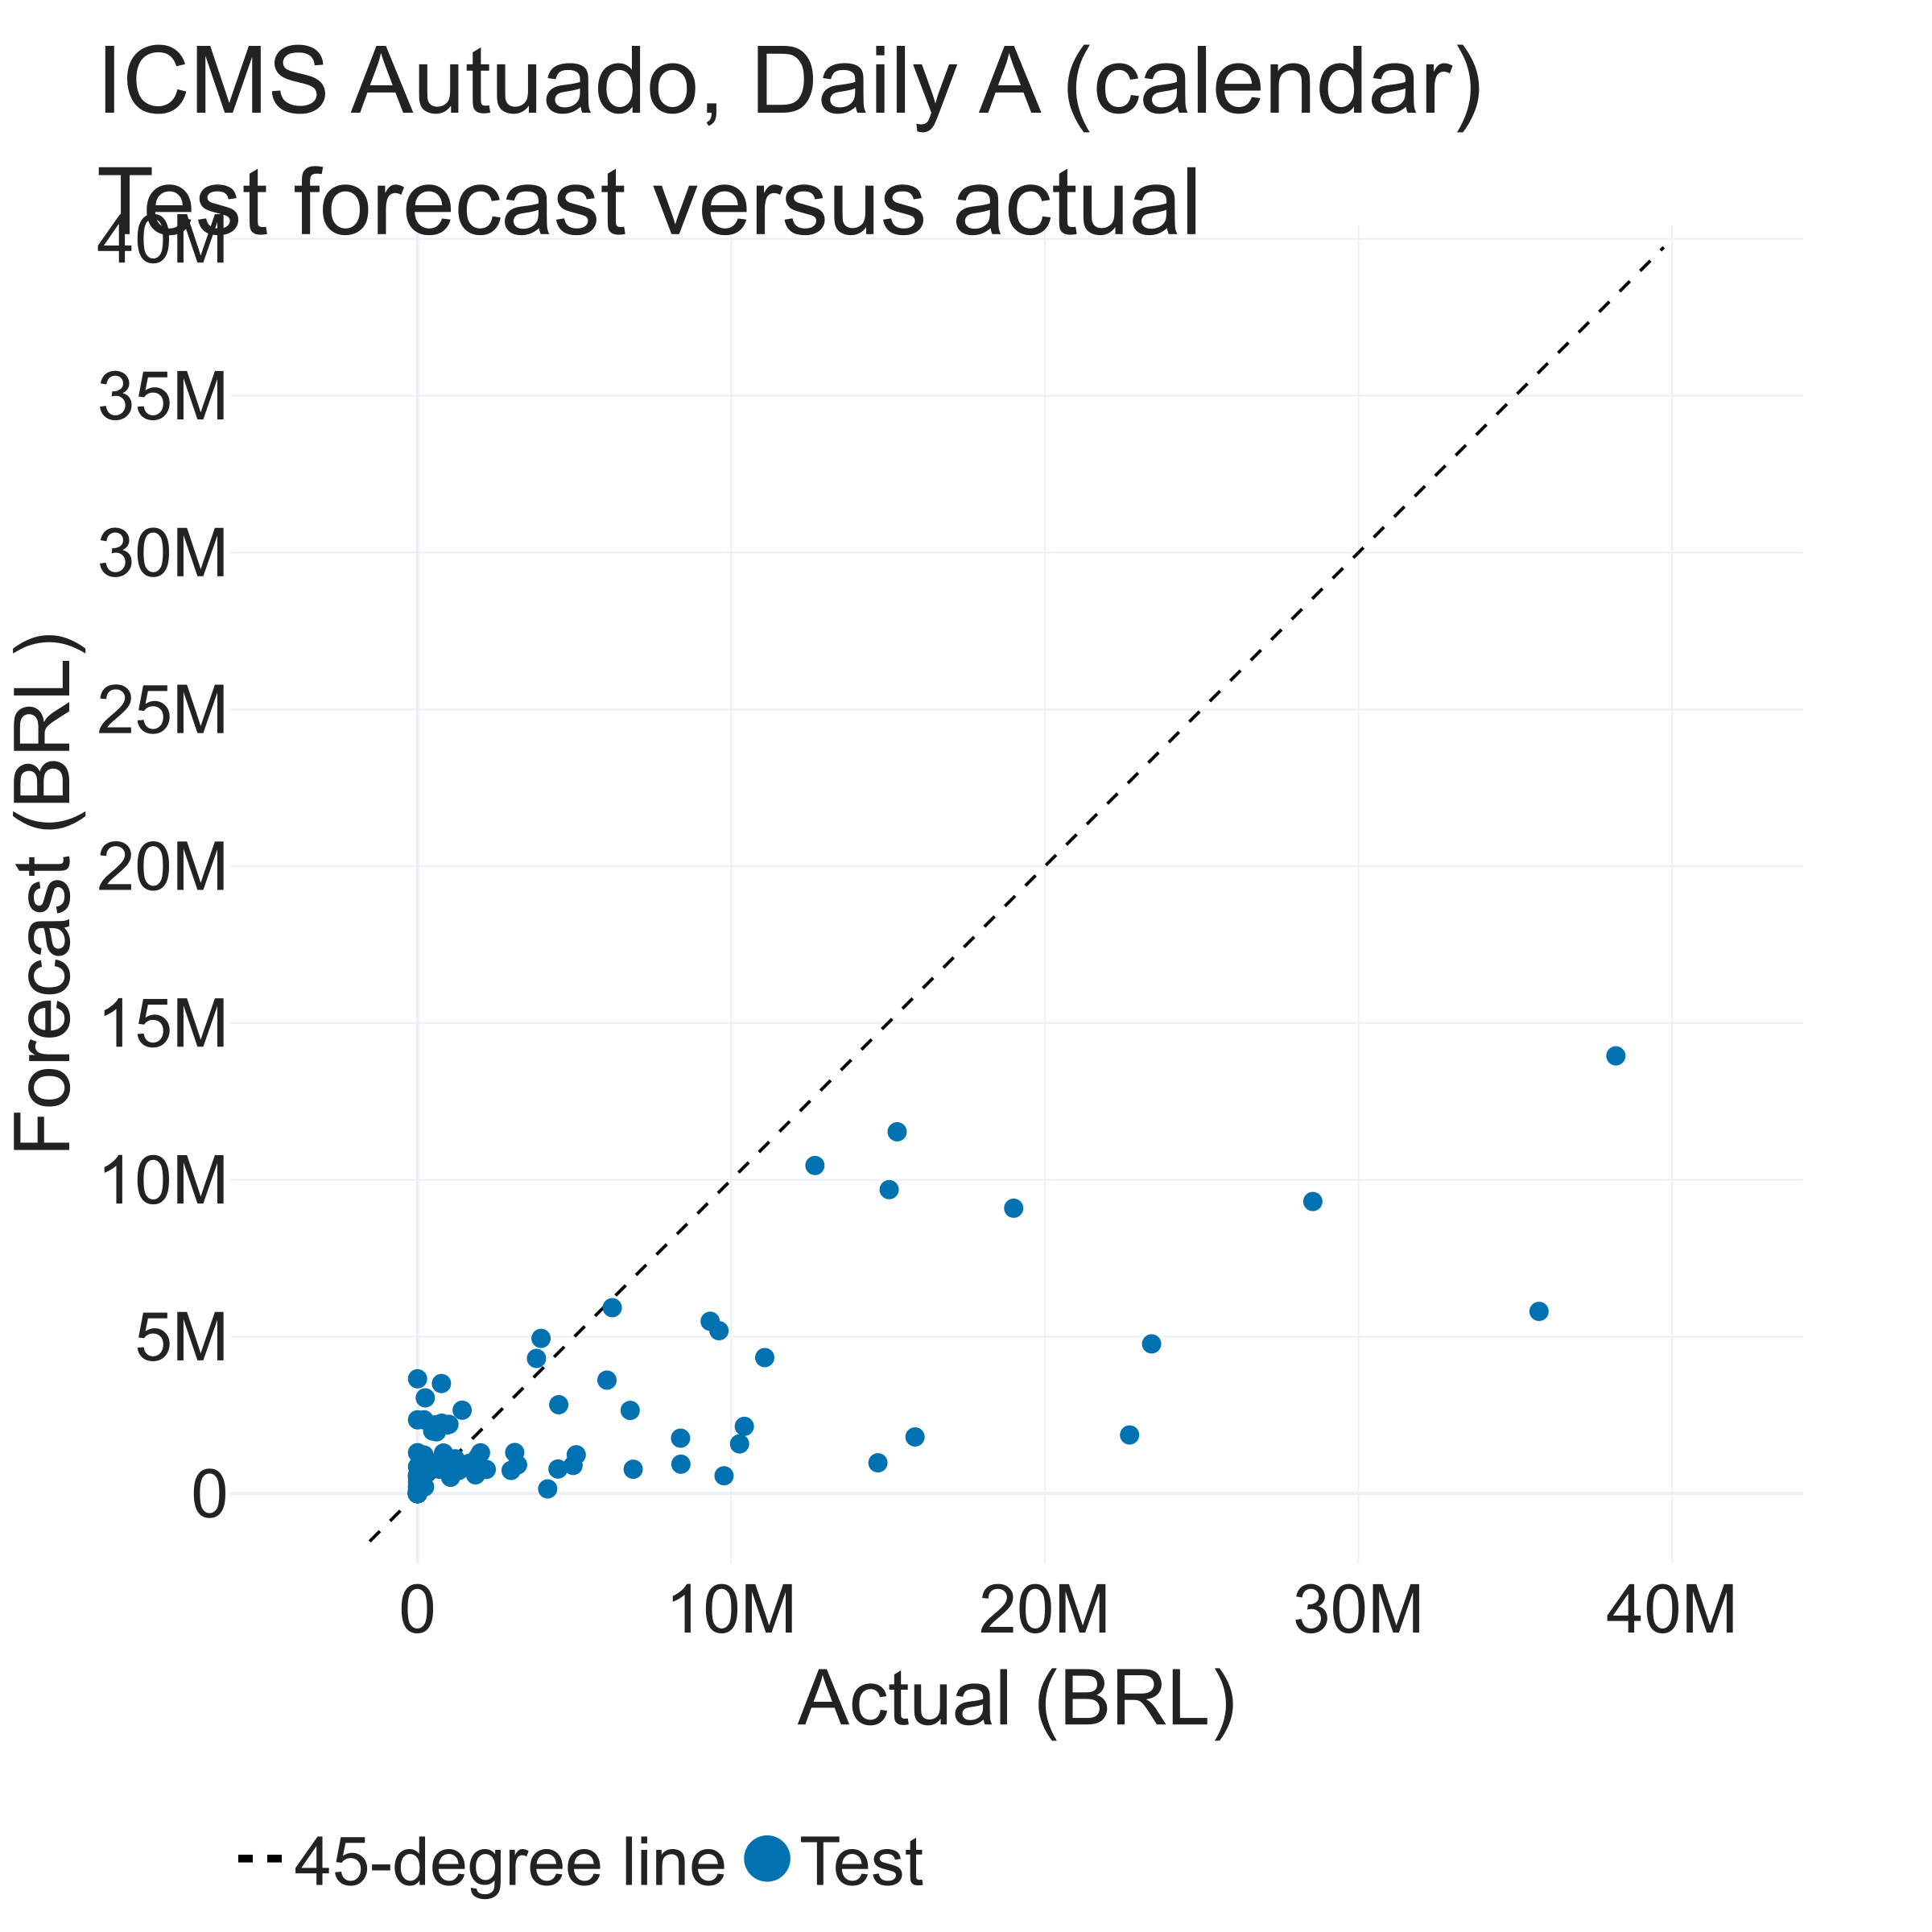
\includegraphics[width=0.62\linewidth]{figures/segment/autuado_daily_scatter.png}
  \caption{Autuado, daily A test scatter.}
\end{figure}
